\documentclass[]{article}
\usepackage{lmodern}
\usepackage{amssymb,amsmath}
\usepackage{ifxetex,ifluatex}
\usepackage{fixltx2e} % provides \textsubscript
\ifnum 0\ifxetex 1\fi\ifluatex 1\fi=0 % if pdftex
  \usepackage[T1]{fontenc}
  \usepackage[utf8]{inputenc}
\else % if luatex or xelatex
  \ifxetex
    \usepackage{mathspec}
  \else
    \usepackage{fontspec}
  \fi
  \defaultfontfeatures{Ligatures=TeX,Scale=MatchLowercase}
\fi
% use upquote if available, for straight quotes in verbatim environments
\IfFileExists{upquote.sty}{\usepackage{upquote}}{}
% use microtype if available
\IfFileExists{microtype.sty}{%
\usepackage{microtype}
\UseMicrotypeSet[protrusion]{basicmath} % disable protrusion for tt fonts
}{}
\usepackage[margin=1in]{geometry}
\usepackage{hyperref}
\hypersetup{unicode=true,
            pdftitle={Homework 02},
            pdfauthor={Weiling Li},
            pdfborder={0 0 0},
            breaklinks=true}
\urlstyle{same}  % don't use monospace font for urls
\usepackage{color}
\usepackage{fancyvrb}
\newcommand{\VerbBar}{|}
\newcommand{\VERB}{\Verb[commandchars=\\\{\}]}
\DefineVerbatimEnvironment{Highlighting}{Verbatim}{commandchars=\\\{\}}
% Add ',fontsize=\small' for more characters per line
\usepackage{framed}
\definecolor{shadecolor}{RGB}{248,248,248}
\newenvironment{Shaded}{\begin{snugshade}}{\end{snugshade}}
\newcommand{\AlertTok}[1]{\textcolor[rgb]{0.94,0.16,0.16}{#1}}
\newcommand{\AnnotationTok}[1]{\textcolor[rgb]{0.56,0.35,0.01}{\textbf{\textit{#1}}}}
\newcommand{\AttributeTok}[1]{\textcolor[rgb]{0.77,0.63,0.00}{#1}}
\newcommand{\BaseNTok}[1]{\textcolor[rgb]{0.00,0.00,0.81}{#1}}
\newcommand{\BuiltInTok}[1]{#1}
\newcommand{\CharTok}[1]{\textcolor[rgb]{0.31,0.60,0.02}{#1}}
\newcommand{\CommentTok}[1]{\textcolor[rgb]{0.56,0.35,0.01}{\textit{#1}}}
\newcommand{\CommentVarTok}[1]{\textcolor[rgb]{0.56,0.35,0.01}{\textbf{\textit{#1}}}}
\newcommand{\ConstantTok}[1]{\textcolor[rgb]{0.00,0.00,0.00}{#1}}
\newcommand{\ControlFlowTok}[1]{\textcolor[rgb]{0.13,0.29,0.53}{\textbf{#1}}}
\newcommand{\DataTypeTok}[1]{\textcolor[rgb]{0.13,0.29,0.53}{#1}}
\newcommand{\DecValTok}[1]{\textcolor[rgb]{0.00,0.00,0.81}{#1}}
\newcommand{\DocumentationTok}[1]{\textcolor[rgb]{0.56,0.35,0.01}{\textbf{\textit{#1}}}}
\newcommand{\ErrorTok}[1]{\textcolor[rgb]{0.64,0.00,0.00}{\textbf{#1}}}
\newcommand{\ExtensionTok}[1]{#1}
\newcommand{\FloatTok}[1]{\textcolor[rgb]{0.00,0.00,0.81}{#1}}
\newcommand{\FunctionTok}[1]{\textcolor[rgb]{0.00,0.00,0.00}{#1}}
\newcommand{\ImportTok}[1]{#1}
\newcommand{\InformationTok}[1]{\textcolor[rgb]{0.56,0.35,0.01}{\textbf{\textit{#1}}}}
\newcommand{\KeywordTok}[1]{\textcolor[rgb]{0.13,0.29,0.53}{\textbf{#1}}}
\newcommand{\NormalTok}[1]{#1}
\newcommand{\OperatorTok}[1]{\textcolor[rgb]{0.81,0.36,0.00}{\textbf{#1}}}
\newcommand{\OtherTok}[1]{\textcolor[rgb]{0.56,0.35,0.01}{#1}}
\newcommand{\PreprocessorTok}[1]{\textcolor[rgb]{0.56,0.35,0.01}{\textit{#1}}}
\newcommand{\RegionMarkerTok}[1]{#1}
\newcommand{\SpecialCharTok}[1]{\textcolor[rgb]{0.00,0.00,0.00}{#1}}
\newcommand{\SpecialStringTok}[1]{\textcolor[rgb]{0.31,0.60,0.02}{#1}}
\newcommand{\StringTok}[1]{\textcolor[rgb]{0.31,0.60,0.02}{#1}}
\newcommand{\VariableTok}[1]{\textcolor[rgb]{0.00,0.00,0.00}{#1}}
\newcommand{\VerbatimStringTok}[1]{\textcolor[rgb]{0.31,0.60,0.02}{#1}}
\newcommand{\WarningTok}[1]{\textcolor[rgb]{0.56,0.35,0.01}{\textbf{\textit{#1}}}}
\usepackage{graphicx,grffile}
\makeatletter
\def\maxwidth{\ifdim\Gin@nat@width>\linewidth\linewidth\else\Gin@nat@width\fi}
\def\maxheight{\ifdim\Gin@nat@height>\textheight\textheight\else\Gin@nat@height\fi}
\makeatother
% Scale images if necessary, so that they will not overflow the page
% margins by default, and it is still possible to overwrite the defaults
% using explicit options in \includegraphics[width, height, ...]{}
\setkeys{Gin}{width=\maxwidth,height=\maxheight,keepaspectratio}
\IfFileExists{parskip.sty}{%
\usepackage{parskip}
}{% else
\setlength{\parindent}{0pt}
\setlength{\parskip}{6pt plus 2pt minus 1pt}
}
\setlength{\emergencystretch}{3em}  % prevent overfull lines
\providecommand{\tightlist}{%
  \setlength{\itemsep}{0pt}\setlength{\parskip}{0pt}}
\setcounter{secnumdepth}{0}
% Redefines (sub)paragraphs to behave more like sections
\ifx\paragraph\undefined\else
\let\oldparagraph\paragraph
\renewcommand{\paragraph}[1]{\oldparagraph{#1}\mbox{}}
\fi
\ifx\subparagraph\undefined\else
\let\oldsubparagraph\subparagraph
\renewcommand{\subparagraph}[1]{\oldsubparagraph{#1}\mbox{}}
\fi

%%% Use protect on footnotes to avoid problems with footnotes in titles
\let\rmarkdownfootnote\footnote%
\def\footnote{\protect\rmarkdownfootnote}

%%% Change title format to be more compact
\usepackage{titling}

% Create subtitle command for use in maketitle
\newcommand{\subtitle}[1]{
  \posttitle{
    \begin{center}\large#1\end{center}
    }
}

\setlength{\droptitle}{-2em}

  \title{Homework 02}
    \pretitle{\vspace{\droptitle}\centering\huge}
  \posttitle{\par}
    \author{Weiling Li}
    \preauthor{\centering\large\emph}
  \postauthor{\par}
      \predate{\centering\large\emph}
  \postdate{\par}
    \date{Septemeber 21, 2019}

\usepackage{booktabs}
\usepackage{longtable}
\usepackage{array}
\usepackage{multirow}
\usepackage{wrapfig}
\usepackage{float}
\usepackage{colortbl}
\usepackage{pdflscape}
\usepackage{tabu}
\usepackage{threeparttable}
\usepackage{threeparttablex}
\usepackage[normalem]{ulem}
\usepackage{makecell}
\usepackage{xcolor}

\begin{document}
\maketitle

\newcommand{\mat}[1]{\boldsymbol{#1}} 
\newcommand{\norm}[1]{\left\lVert#1\right\rVert}
\newcommand{\rv}[1]{\underline{#1}}

\hypertarget{introduction}{%
\section{Introduction}\label{introduction}}

In homework 2 you will fit many regression models. You are welcome to
explore beyond what the question is asking you.

Please come see us we are here to help.

\hypertarget{data-analysis}{%
\subsection{Data analysis}\label{data-analysis}}

\hypertarget{analysis-of-earnings-and-height-data}{%
\subsubsection{Analysis of earnings and height
data}\label{analysis-of-earnings-and-height-data}}

The folder \texttt{earnings} has data from the Work, Family, and
Well-Being Survey (Ross, 1990). You can find the codebook at
\url{http://www.stat.columbia.edu/~gelman/arm/examples/earnings/wfwcodebook.txt}

\begin{Shaded}
\begin{Highlighting}[]
\NormalTok{gelman_dir <-}\StringTok{ "http://www.stat.columbia.edu/~gelman/arm/examples/"}
\NormalTok{heights    <-}\StringTok{ }\KeywordTok{read.dta}\NormalTok{ (}\KeywordTok{paste0}\NormalTok{(gelman_dir,}\StringTok{"earnings/heights.dta"}\NormalTok{))}
\CommentTok{#wfw90    <- read.table (paste0(gelman_dir,"earnings/wfw90.dat"))}
\end{Highlighting}
\end{Shaded}

Pull out the data on earnings, sex, height, and weight.

\begin{enumerate}
\def\labelenumi{\arabic{enumi}.}
\tightlist
\item
  In R, check the dataset and clean any unusually coded data.
\end{enumerate}

The dataset has 9 variables, from the code book, they mean the
following:

\begin{itemize}
\item
  earn: personal income during year 1989, in dollars.

  \begin{itemize}
  \tightlist
  \item
    height1: height in inches \%/\% 12.
  \item
    height2: height in inches \%\% 12.
  \end{itemize}
\item
  sex:

  \begin{itemize}
  \tightlist
  \item
    male: 1
  \item
    female: 2
  \end{itemize}
\item
  race:

  \begin{itemize}
  \tightlist
  \item
    white: 1
  \item
    black: 2
  \item
    asian: 3
  \item
    native amerian: 4
  \item
    others: 9
  \end{itemize}
\item
  hisp:

  \begin{itemize}
  \tightlist
  \item
    hispanic origin: 1
  \item
    otherwise: 2
  \end{itemize}
\item
  highest grade or years in school(highest grade converted to years in
  school) from 0 to 18, integers.
\item
  yearbn: year of born in 19xx.
\item
  height: interviewee's height in inches, rounded to nearest integer.
\end{itemize}

\newline

\begin{Shaded}
\begin{Highlighting}[]
\CommentTok{## Earnings has NA value and 0 value, which needs to be cleaned. }
\CommentTok{## Also, to better managing data. original data had been put in tibble form.}
\CommentTok{## For the purpose of this HW, only earn,sex,race,ed & height were kept}
\NormalTok{h1 <-}\StringTok{ }\KeywordTok{filter}\NormalTok{(}\KeywordTok{filter}\NormalTok{(}\KeywordTok{as_tibble}\NormalTok{(heights),}\OperatorTok{!}\KeywordTok{is.na}\NormalTok{(earn)),earn }\OperatorTok{>}\DecValTok{0}\NormalTok{)}\OperatorTok\KeywordTok{select}\NormalTok{(earn,sex,race,yearbn,ed,height)}
\end{Highlighting}
\end{Shaded}

\begin{verbatim}
## Warning: `lang()` is deprecated as of rlang 0.2.0.
## Please use `call2()` instead.
## This warning is displayed once per session.
\end{verbatim}

\begin{verbatim}
## Warning: `new_overscope()` is deprecated as of rlang 0.2.0.
## Please use `new_data_mask()` instead.
## This warning is displayed once per session.
\end{verbatim}

\begin{verbatim}
## Warning: `overscope_eval_next()` is deprecated as of rlang 0.2.0.
## Please use `eval_tidy()` with a data mask instead.
## This warning is displayed once per session.
\end{verbatim}

\begin{Shaded}
\begin{Highlighting}[]
\CommentTok{#hist(log(h1$earn),probability = T)}
\CommentTok{#hist(h1$ed,probability = T)}
\CommentTok{#hist(h1$height,probability = T)}
\end{Highlighting}
\end{Shaded}

\begin{enumerate}
\def\labelenumi{\arabic{enumi}.}
\setcounter{enumi}{1}
\tightlist
\item
  Fit a linear regression model predicting earnings from height. What
  transformation should you perform in order to interpret the intercept
  from this model as average earnings for people with average height?
\end{enumerate}

\begin{Shaded}
\begin{Highlighting}[]
\CommentTok{#to achieve what exactly asked. we only need to subtract height with mean.}
\NormalTok{h1 <-}\StringTok{ }\KeywordTok{mutate}\NormalTok{(h1,}\DataTypeTok{h.centered =}\NormalTok{ height }\OperatorTok{-}\StringTok{ }\KeywordTok{mean}\NormalTok{(h1}\OperatorTok{$}\NormalTok{height))}
\end{Highlighting}
\end{Shaded}

\begin{verbatim}
## Warning: The `printer` argument is deprecated as of rlang 0.3.0.
## This warning is displayed once per session.
\end{verbatim}

\begin{Shaded}
\begin{Highlighting}[]
\CommentTok{#hist(height.centered)}
\CommentTok{#hist(h1$height)}
\KeywordTok{ggplot}\NormalTok{(h1)}\OperatorTok{+}
\StringTok{  }\KeywordTok{aes}\NormalTok{(}\DataTypeTok{x =}\NormalTok{ h.centered, }\DataTypeTok{y =}\NormalTok{ earn)}\OperatorTok{+}\KeywordTok{geom_point}\NormalTok{()}\OperatorTok{+}\KeywordTok{geom_smooth}\NormalTok{(}\DataTypeTok{method =} \StringTok{'lm'}\NormalTok{,}\DataTypeTok{se =}\NormalTok{ F)}\OperatorTok{+}\KeywordTok{ggtitle}\NormalTok{(}\KeywordTok{paste0}\NormalTok{(}\StringTok{'intercept = '}\NormalTok{,}\KeywordTok{toString}\NormalTok{(}\KeywordTok{round}\NormalTok{(}\KeywordTok{coef}\NormalTok{(}\KeywordTok{lm}\NormalTok{(}\DataTypeTok{data =}\NormalTok{ h1, earn }\OperatorTok{~}\StringTok{ }\NormalTok{h.centered))[}\DecValTok{1}\NormalTok{],}\DecValTok{2}\NormalTok{))))}\OperatorTok{+}\KeywordTok{theme}\NormalTok{(}\DataTypeTok{plot.title =} \KeywordTok{element_text}\NormalTok{(}\DataTypeTok{size =} \DecValTok{28}\NormalTok{,}\DataTypeTok{hjust =} \FloatTok{.5}\NormalTok{))}
\end{Highlighting}
\end{Shaded}

\begin{center}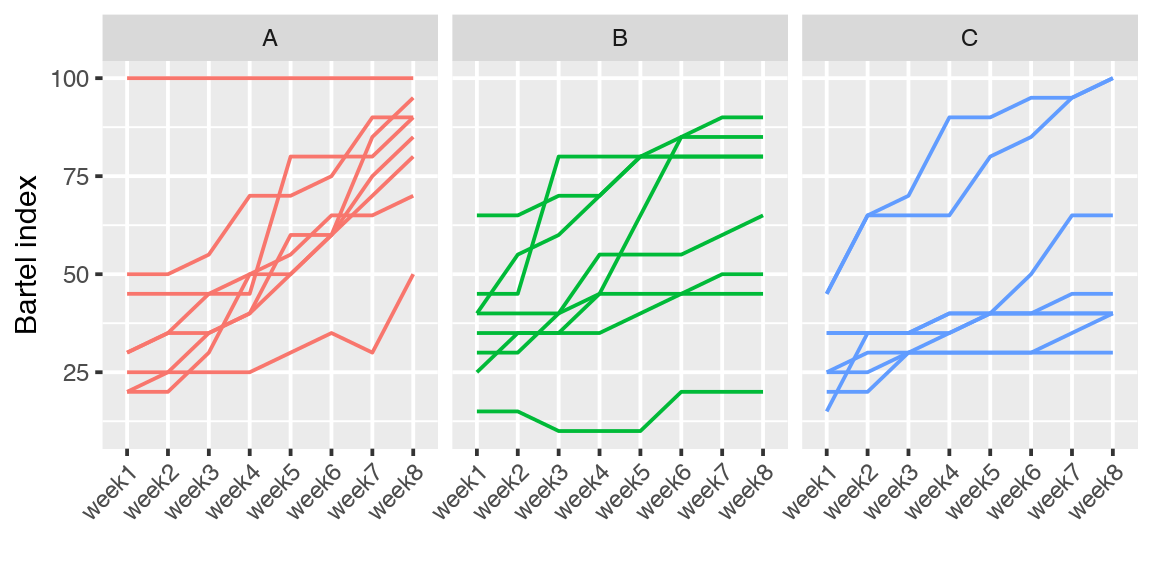
\includegraphics{hw_linear_reg_2_files/figure-latex/unnamed-chunk-3-1} \end{center}

\begin{Shaded}
\begin{Highlighting}[]
\CommentTok{#however, as can be seen from the residual plot and the histogram of earn, the skewness of the earn causes the residual to be distributed unevenly}
\KeywordTok{ggplot}\NormalTok{(h1)}\OperatorTok{+}\KeywordTok{aes}\NormalTok{(}\DataTypeTok{x =}\NormalTok{ earn)}\OperatorTok{+}\KeywordTok{geom_histogram}\NormalTok{(}\DataTypeTok{bins =} \DecValTok{30}\NormalTok{,}\DataTypeTok{alpha =} \FloatTok{.4}\NormalTok{,}\KeywordTok{aes}\NormalTok{(}\DataTypeTok{y=}\NormalTok{..density..))}\OperatorTok{+}\KeywordTok{geom_density}\NormalTok{()}
\end{Highlighting}
\end{Shaded}

\begin{center}\includegraphics{hw_linear_reg_2_files/figure-latex/unnamed-chunk-3-2} \end{center}

\begin{Shaded}
\begin{Highlighting}[]
\KeywordTok{ggplot}\NormalTok{(}\KeywordTok{lm}\NormalTok{(}\DataTypeTok{data =}\NormalTok{ h1, earn }\OperatorTok{~}\StringTok{ }\NormalTok{h.centered)) }\OperatorTok{+}\StringTok{ }\KeywordTok{aes}\NormalTok{(}\DataTypeTok{x=}\NormalTok{.fitted, }\DataTypeTok{y=}\NormalTok{.resid)}\OperatorTok{+}
\StringTok{  }\KeywordTok{geom_point}\NormalTok{()}\OperatorTok{+}\KeywordTok{geom_abline}\NormalTok{(}\DataTypeTok{intercept =} \DecValTok{0}\NormalTok{,}\DataTypeTok{slope =} \DecValTok{0}\NormalTok{,}\DataTypeTok{color=}\StringTok{'orange'}\NormalTok{,}\DataTypeTok{size=}\DecValTok{1}\NormalTok{)}\OperatorTok{+}\KeywordTok{geom_smooth}\NormalTok{(}\DataTypeTok{method =} \StringTok{'loess'}\NormalTok{,}\DataTypeTok{alpha =} \FloatTok{.4}\NormalTok{)}
\end{Highlighting}
\end{Shaded}

\begin{center}\includegraphics{hw_linear_reg_2_files/figure-latex/unnamed-chunk-3-3} \end{center}

\begin{Shaded}
\begin{Highlighting}[]
\CommentTok{#this violates the assumption of linear regression, to better achieve the results. One should at 1st regularize the earning, by taking a log transformation, the skewness issue had been greatly improved.}
\end{Highlighting}
\end{Shaded}

\begin{enumerate}
\def\labelenumi{\arabic{enumi}.}
\setcounter{enumi}{2}
\tightlist
\item
  Fit some regression models with the goal of predicting earnings from
  some combination of sex, height, and age. Be sure to try various
  transformations and interactions that might make sense. Choose your
  preferred model and justify.\\
  census data:
  \href{https://www2.census.gov/library/publications/decennial/1990/cp-1/cp-1-1.pdf\#}{us
  1990 census}\newline codebook:
  \href{http://www.stat.columbia.edu/~gelman/arm/examples/earnings/wfwcodebook.txt}{wfwcodebook.txt}\newline
\end{enumerate}

\begin{Shaded}
\begin{Highlighting}[]
\CommentTok{## for better interpretation and simplicity, the following transformation of the data set is done as follows:}
\CommentTok{## take log transformation of the earning}
\CommentTok{## substract sex with 1 to make the variable a binary with 0 indicate male and 1 indicate female.}
\CommentTok{## 90 - yearbn to get the approximate age for the interviewee as they report their earning. to ensure no negative value occurs, for yearbn>72, we use 190 - yearbn(The sample was taken in a way that it only collects information from individuals older than 18. thus any age less than 18 was resulted by birth year before 1900)}
\NormalTok{h.transformed <-}\StringTok{ }\KeywordTok{mutate}\NormalTok{(h1,}\DataTypeTok{log.earn =} \KeywordTok{log}\NormalTok{(earn)) }\OperatorTok\StringTok{ }\KeywordTok{mutate}\NormalTok{(}\DataTypeTok{sex =}\NormalTok{ sex }\OperatorTok{-}\StringTok{ }\DecValTok{1}\NormalTok{) }\OperatorTok\StringTok{ }\KeywordTok{mutate}\NormalTok{(}\DataTypeTok{age =} \KeywordTok{ifelse}\NormalTok{(yearbn}\OperatorTok{>}\DecValTok{72}\NormalTok{, }\DecValTok{190} \OperatorTok{-}\StringTok{ }\NormalTok{yearbn,}\DecValTok{90} \OperatorTok{-}\StringTok{ }\NormalTok{yearbn))}
\CommentTok{## A sample of the transformed data is shown below}
\KeywordTok{kable}\NormalTok{(}\KeywordTok{sample_n}\NormalTok{(h.transformed,}\DecValTok{10}\NormalTok{,}\DataTypeTok{replace =}\NormalTok{ T)}\OperatorTok\KeywordTok{select}\NormalTok{(log.earn,sex,h.centered,age),}\DataTypeTok{format =} \StringTok{'html'}\NormalTok{,}\DataTypeTok{digits =} \DecValTok{2}\NormalTok{)}
\end{Highlighting}
\end{Shaded}

log.earn

sex

h.centered

age

9.21

1

1.08

56

10.71

1

-0.92

43

9.62

0

5.08

40

9.68

1

-3.92

27

10.55

0

1.08

46

10.31

0

0.08

31

9.10

0

0.08

33

10.17

1

2.08

43

9.85

0

5.08

28

11.00

1

-0.92

43

\begin{Shaded}
\begin{Highlighting}[]
\CommentTok{##check race factor:}
\KeywordTok{kable}\NormalTok{(}\KeywordTok{group_by}\NormalTok{(h.transformed,race)}\OperatorTok\KeywordTok{summarise}\NormalTok{(}\DataTypeTok{count.race =} \KeywordTok{n}\NormalTok{()),}\DataTypeTok{format =} \StringTok{'html'}\NormalTok{)}
\end{Highlighting}
\end{Shaded}

race

count.race

1

1051

2

112

3

15

4

11

9

3

\begin{Shaded}
\begin{Highlighting}[]
\CommentTok{## as can be seen the majority interviewees are white, less than 10% are black and less than 2% are other races. }
\CommentTok{## The 1990 census data shows that about 80% american population is white, 12% is black and the remaining is considered others. from this stand point. besides the white population is over represented in the sample survey and other races under-represented. From the race stand point, the sample is valid. However, because the observations of races other than white is too low, spliting the data by race is not a good idea. One should do either an analysis on white only or ignore the race factor.}
\CommentTok{#ggplot(h.transformed)+aes(x = h.centered,y = log.earn,color = as.factor(sex))+geom_point()+geom_smooth(method='lm',se = F)}

\CommentTok{## Lets see how our variables natrually distributed under gender factors}
\CommentTok{## height}
\KeywordTok{ggplot}\NormalTok{(h.transformed)}\OperatorTok{+}\KeywordTok{aes}\NormalTok{(}\DataTypeTok{x =}\NormalTok{ h.centered,}\DataTypeTok{color =} \KeywordTok{as.factor}\NormalTok{(sex))}\OperatorTok{+}\KeywordTok{geom_density}\NormalTok{( }\DataTypeTok{alpha =} \FloatTok{.4}\NormalTok{)}\OperatorTok{+}\KeywordTok{geom_histogram}\NormalTok{(}\DataTypeTok{bins =} \DecValTok{30}\NormalTok{,}\DataTypeTok{alpha =} \FloatTok{.4}\NormalTok{,}\KeywordTok{aes}\NormalTok{(}\DataTypeTok{y=}\NormalTok{..density..),}\DataTypeTok{fill =} \OtherTok{NA}\NormalTok{ )}
\end{Highlighting}
\end{Shaded}

\begin{center}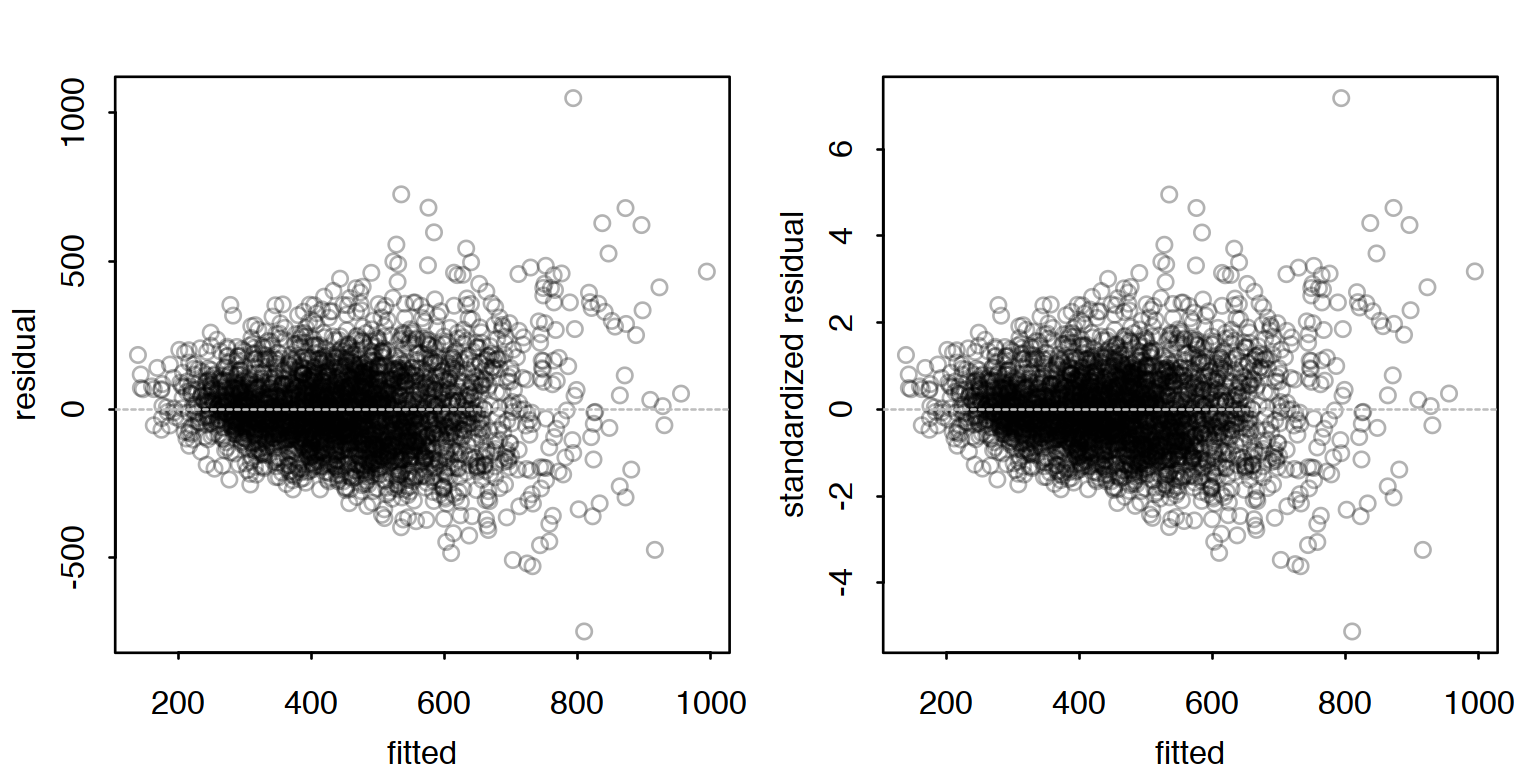
\includegraphics{hw_linear_reg_2_files/figure-latex/unnamed-chunk-4-1} \end{center}

\begin{Shaded}
\begin{Highlighting}[]
\KeywordTok{ggplot}\NormalTok{(h.transformed)}\OperatorTok{+}\KeywordTok{aes}\NormalTok{(}\DataTypeTok{x =}\NormalTok{ h.centered,}\DataTypeTok{y =}\NormalTok{ log.earn,}\DataTypeTok{color =} \KeywordTok{as.factor}\NormalTok{(sex))}\OperatorTok{+}\KeywordTok{geom_jitter}\NormalTok{()}\OperatorTok{+}\KeywordTok{geom_smooth}\NormalTok{(}\DataTypeTok{method=}\StringTok{'loess'}\NormalTok{)}
\end{Highlighting}
\end{Shaded}

\begin{center}\includegraphics{hw_linear_reg_2_files/figure-latex/unnamed-chunk-4-2} \end{center}

\begin{Shaded}
\begin{Highlighting}[]
\CommentTok{## age}
\KeywordTok{ggplot}\NormalTok{(h.transformed)}\OperatorTok{+}\KeywordTok{aes}\NormalTok{(}\DataTypeTok{x =}\NormalTok{ age,}\DataTypeTok{color =} \KeywordTok{as.factor}\NormalTok{(sex))}\OperatorTok{+}\KeywordTok{geom_density}\NormalTok{( }\DataTypeTok{alpha =} \FloatTok{.4}\NormalTok{)}\OperatorTok{+}\KeywordTok{geom_histogram}\NormalTok{(}\DataTypeTok{bins =} \DecValTok{30}\NormalTok{,}\DataTypeTok{alpha =} \FloatTok{.4}\NormalTok{,}\KeywordTok{aes}\NormalTok{(}\DataTypeTok{y=}\NormalTok{..density..),}\DataTypeTok{fill =} \OtherTok{NA}\NormalTok{ )}
\end{Highlighting}
\end{Shaded}

\begin{center}\includegraphics{hw_linear_reg_2_files/figure-latex/unnamed-chunk-4-3} \end{center}

\begin{Shaded}
\begin{Highlighting}[]
\KeywordTok{ggplot}\NormalTok{(h.transformed)}\OperatorTok{+}\KeywordTok{aes}\NormalTok{(}\DataTypeTok{x =}\NormalTok{ age,}\DataTypeTok{y =}\NormalTok{ log.earn,}\DataTypeTok{color =} \KeywordTok{as.factor}\NormalTok{(sex))}\OperatorTok{+}\KeywordTok{geom_jitter}\NormalTok{()}\OperatorTok{+}\KeywordTok{geom_smooth}\NormalTok{(}\DataTypeTok{method=}\StringTok{'loess'}\NormalTok{)}
\end{Highlighting}
\end{Shaded}

\begin{center}\includegraphics{hw_linear_reg_2_files/figure-latex/unnamed-chunk-4-4} \end{center}

\begin{Shaded}
\begin{Highlighting}[]
\CommentTok{## education}
\KeywordTok{ggplot}\NormalTok{(h.transformed)}\OperatorTok{+}\KeywordTok{aes}\NormalTok{(}\DataTypeTok{x =}\NormalTok{ ed,}\DataTypeTok{color =} \KeywordTok{as.factor}\NormalTok{(sex))}\OperatorTok{+}\KeywordTok{geom_density}\NormalTok{( }\DataTypeTok{alpha =} \FloatTok{.4}\NormalTok{)}\OperatorTok{+}\KeywordTok{geom_histogram}\NormalTok{(}\DataTypeTok{bins =} \DecValTok{30}\NormalTok{,}\DataTypeTok{alpha =} \FloatTok{.4}\NormalTok{,}\KeywordTok{aes}\NormalTok{(}\DataTypeTok{y=}\NormalTok{..density..),}\DataTypeTok{fill =} \OtherTok{NA}\NormalTok{ )}
\end{Highlighting}
\end{Shaded}

\begin{center}\includegraphics{hw_linear_reg_2_files/figure-latex/unnamed-chunk-4-5} \end{center}

\begin{Shaded}
\begin{Highlighting}[]
\KeywordTok{ggplot}\NormalTok{(h.transformed)}\OperatorTok{+}\KeywordTok{aes}\NormalTok{(}\DataTypeTok{x =}\NormalTok{ ed,}\DataTypeTok{y =}\NormalTok{ log.earn,}\DataTypeTok{color =} \KeywordTok{as.factor}\NormalTok{(sex))}\OperatorTok{+}\KeywordTok{geom_jitter}\NormalTok{()}\OperatorTok{+}\KeywordTok{geom_smooth}\NormalTok{(}\DataTypeTok{method=}\StringTok{'loess'}\NormalTok{)}
\end{Highlighting}
\end{Shaded}

\begin{center}\includegraphics{hw_linear_reg_2_files/figure-latex/unnamed-chunk-4-6} \end{center}

One can observed from the histogram that height variable is unevenly
distributed between genders. female has a mean roughly 3 inches below
average while male roughly 4 inches above average with both genders have
an approximated sample standard error at 2.5 inches. This fact
approximately puts the mean of one gender out of 2 standard errors of
the opposite gender. in this case, when we are predicting using height
variable, we inevitably have to use gender to separate them. Also,
because gender had seperated heights into two clusters, it is better to
introduce interaction terms \(height \times gender\) to ensure linear
regression models the two genders differently. \newline The model's
coefficient and it's residual plots was given below:\newline

\begin{Shaded}
\begin{Highlighting}[]
\NormalTok{MD1 =}\StringTok{ }\KeywordTok{lm}\NormalTok{(}\DataTypeTok{data =}\NormalTok{ h.transformed,log.earn }\OperatorTok{~}\StringTok{ }\NormalTok{sex }\OperatorTok{+}\StringTok{ }\NormalTok{h.centered }\OperatorTok{+}\StringTok{ }\NormalTok{sex}\OperatorTok{*}\NormalTok{h.centered)}
\KeywordTok{summary}\NormalTok{(MD1)}\OperatorTok{$}\NormalTok{call}
\end{Highlighting}
\end{Shaded}

\begin{verbatim}
## lm(formula = log.earn ~ sex + h.centered + sex * h.centered, 
##     data = h.transformed)
\end{verbatim}

\begin{Shaded}
\begin{Highlighting}[]
\KeywordTok{summary}\NormalTok{(}\KeywordTok{summary}\NormalTok{(MD1))}
\end{Highlighting}
\end{Shaded}

\begin{verbatim}
##               Length Class  Mode   
## call             3   -none- call   
## terms            3   terms  call   
## residuals     1192   -none- numeric
## coefficients    16   -none- numeric
## aliased          4   -none- logical
## sigma            1   -none- numeric
## df               3   -none- numeric
## r.squared        1   -none- numeric
## adj.r.squared    1   -none- numeric
## fstatistic       3   -none- numeric
## cov.unscaled    16   -none- numeric
\end{verbatim}

\begin{Shaded}
\begin{Highlighting}[]
\KeywordTok{summary}\NormalTok{(MD1)}\OperatorTok{$}\NormalTok{coef}
\end{Highlighting}
\end{Shaded}

\begin{verbatim}
##                    Estimate Std. Error    t value     Pr(>|t|)
## (Intercept)     9.946321548 0.05736331 173.391704 0.000000e+00
## sex            -0.419713073 0.07301657  -5.748190 1.145709e-08
## h.centered      0.024454484 0.01330615   1.837834 6.633649e-02
## sex:h.centered -0.007446534 0.01863502  -0.399599 6.895237e-01
\end{verbatim}

\begin{Shaded}
\begin{Highlighting}[]
\KeywordTok{summary}\NormalTok{(MD1)}\OperatorTok{$}\NormalTok{r.squared}
\end{Highlighting}
\end{Shaded}

\begin{verbatim}
## [1] 0.08668346
\end{verbatim}

\begin{Shaded}
\begin{Highlighting}[]
\KeywordTok{summary}\NormalTok{(MD1)}\OperatorTok{$}\NormalTok{call}
\end{Highlighting}
\end{Shaded}

\begin{verbatim}
## lm(formula = log.earn ~ sex + h.centered + sex * h.centered, 
##     data = h.transformed)
\end{verbatim}

\begin{Shaded}
\begin{Highlighting}[]
\KeywordTok{summary}\NormalTok{(MD1)}
\end{Highlighting}
\end{Shaded}

\begin{verbatim}
## 
## Call:
## lm(formula = log.earn ~ sex + h.centered + sex * h.centered, 
##     data = h.transformed)
## 
## Residuals:
##     Min      1Q  Median      3Q     Max 
## -4.2297 -0.3720  0.1388  0.5646  2.2940 
## 
## Coefficients:
##                 Estimate Std. Error t value Pr(>|t|)    
## (Intercept)     9.946322   0.057363 173.392  < 2e-16 ***
## sex            -0.419713   0.073017  -5.748 1.15e-08 ***
## h.centered      0.024454   0.013306   1.838   0.0663 .  
## sex:h.centered -0.007447   0.018635  -0.400   0.6895    
## ---
## Signif. codes:  0 '***' 0.001 '**' 0.01 '*' 0.05 '.' 0.1 ' ' 1
## 
## Residual standard error: 0.8812 on 1188 degrees of freedom
## Multiple R-squared:  0.08668,    Adjusted R-squared:  0.08438 
## F-statistic: 37.58 on 3 and 1188 DF,  p-value: < 2.2e-16
\end{verbatim}

\begin{Shaded}
\begin{Highlighting}[]
\KeywordTok{plot}\NormalTok{(MD1,}\DataTypeTok{which=}\DecValTok{1}\OperatorTok{:}\DecValTok{2}\NormalTok{)}
\end{Highlighting}
\end{Shaded}

\begin{center}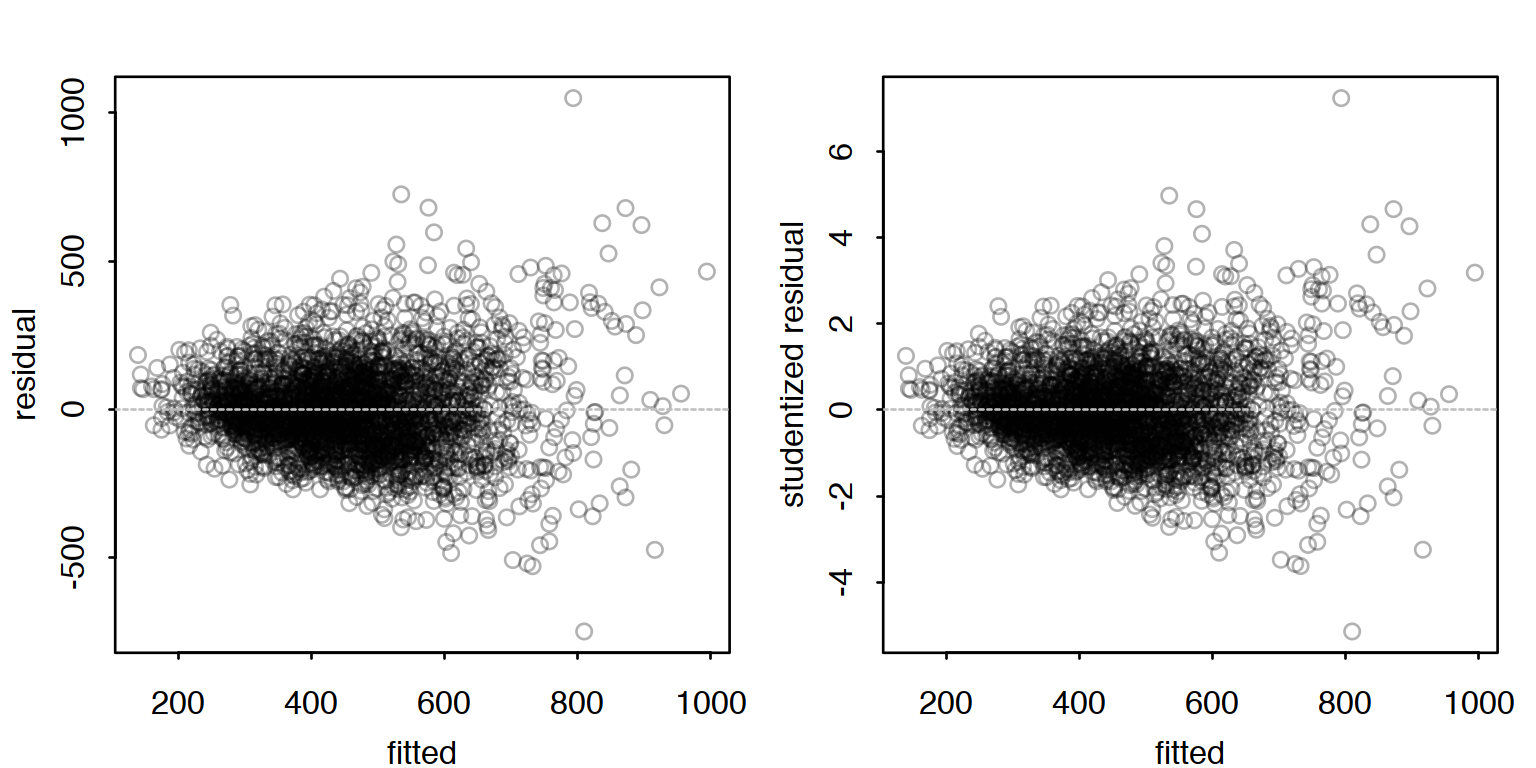
\includegraphics{hw_linear_reg_2_files/figure-latex/unnamed-chunk-5-1} \end{center}

\begin{center}\includegraphics{hw_linear_reg_2_files/figure-latex/unnamed-chunk-5-2} \end{center}

\begin{Shaded}
\begin{Highlighting}[]
\KeywordTok{ggplot}\NormalTok{(h.transformed)}\OperatorTok{+}\KeywordTok{aes}\NormalTok{(}\DataTypeTok{x =}\NormalTok{ h.centered,}\DataTypeTok{y =}\NormalTok{ log.earn,}\DataTypeTok{color =} \KeywordTok{as.factor}\NormalTok{(sex))}\OperatorTok{+}\KeywordTok{geom_jitter}\NormalTok{()}\OperatorTok{+}\KeywordTok{geom_smooth}\NormalTok{(}\DataTypeTok{method=}\StringTok{'lm'}\NormalTok{,}\DataTypeTok{se =}\NormalTok{ F)}
\end{Highlighting}
\end{Shaded}

\begin{center}\includegraphics{hw_linear_reg_2_files/figure-latex/unnamed-chunk-5-3} \end{center}

From the plot shown, the residual show a tiny bias but stays really
close to 0, but the variance is quite high and not equal across all the
heights. From the QQ-plot we can see that the model works reasonably
well for higher height values but have problems with lower height
values.\newline From the age vs log.earn plot we can clearly see that
there can be a nonlinear relationship between the two, for comparison we
construct the model 2 as
\(y = gender + age + age^2 + gender * age + gender * age^2\). \newline

\begin{Shaded}
\begin{Highlighting}[]
\CommentTok{## substract age with min(age) & add one colomn age^2}
\NormalTok{h.transformed <-}\StringTok{ }\KeywordTok{mutate}\NormalTok{(h.transformed,}\DataTypeTok{age =}\NormalTok{ age}\OperatorTok{-}\KeywordTok{min}\NormalTok{(age))}\OperatorTok\KeywordTok{mutate}\NormalTok{(}\DataTypeTok{agesq =}\NormalTok{ age}\OperatorTok{^}\DecValTok{2}\NormalTok{)}
\NormalTok{MD2 =}\StringTok{ }\KeywordTok{lm}\NormalTok{(}\DataTypeTok{data =}\NormalTok{ h.transformed, log.earn }\OperatorTok{~}\StringTok{ }\NormalTok{sex }\OperatorTok{+}\StringTok{ }\NormalTok{age }\OperatorTok{+}\StringTok{ }\NormalTok{agesq }\OperatorTok{+}\StringTok{ }\NormalTok{sex}\OperatorTok{*}\NormalTok{age }\OperatorTok{+}\StringTok{ }\NormalTok{sex }\OperatorTok{*}\NormalTok{agesq)}
\KeywordTok{summary}\NormalTok{(MD2)}\OperatorTok{$}\NormalTok{coef[,}\DecValTok{1}\NormalTok{]}
\end{Highlighting}
\end{Shaded}

\begin{verbatim}
##   (Intercept)           sex           age         agesq       sex:age 
##  9.0601894067 -0.1091444448  0.0872425976 -0.0013161904 -0.0407576635 
##     sex:agesq 
##  0.0006137022
\end{verbatim}

\begin{Shaded}
\begin{Highlighting}[]
\NormalTok{md2coef <-}\StringTok{ }\KeywordTok{summary}\NormalTok{(MD2)}\OperatorTok{$}\NormalTok{coef[,}\DecValTok{1}\NormalTok{]}
\KeywordTok{summary}\NormalTok{(MD2)}\OperatorTok{$}\NormalTok{r.squared}
\end{Highlighting}
\end{Shaded}

\begin{verbatim}
## [1] 0.19855
\end{verbatim}

\begin{Shaded}
\begin{Highlighting}[]
\KeywordTok{plot}\NormalTok{(MD2,}\DataTypeTok{which =} \DecValTok{1}\OperatorTok{:}\DecValTok{2}\NormalTok{)}
\end{Highlighting}
\end{Shaded}

\begin{center}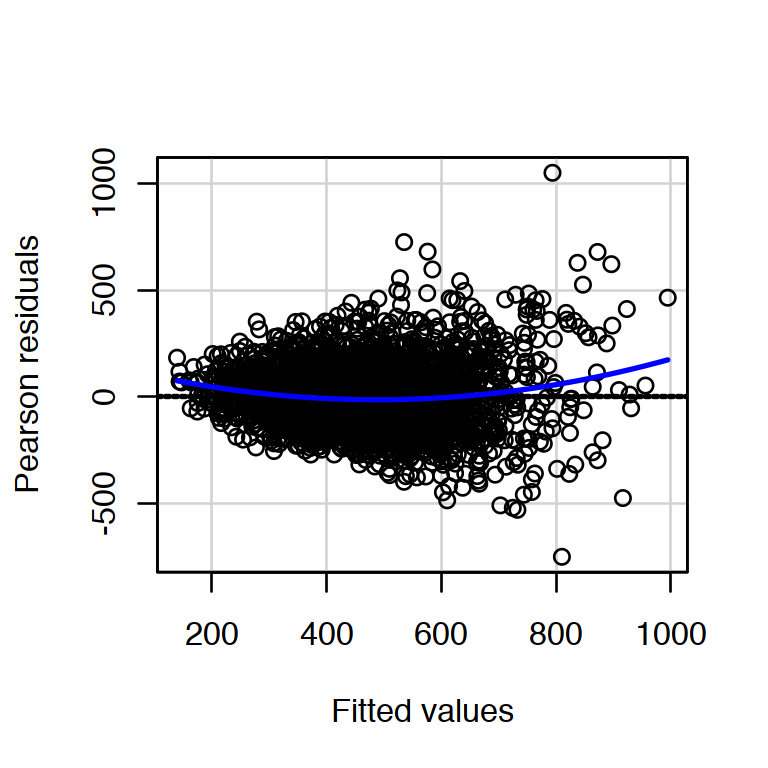
\includegraphics{hw_linear_reg_2_files/figure-latex/unnamed-chunk-6-1} \end{center}

\begin{center}\includegraphics{hw_linear_reg_2_files/figure-latex/unnamed-chunk-6-2} \end{center}

\begin{enumerate}
\def\labelenumi{\arabic{enumi}.}
\setcounter{enumi}{3}
\tightlist
\item
  Interpret all model coefficients. Both models discussed above shows
  although using different variables, but shows a similar results in
  residual analysis. Thus, for the purpose of this HW, model 2 using age
  \& gender is selected to interpret here.\newline
\end{enumerate}

\begin{Shaded}
\begin{Highlighting}[]
\KeywordTok{kable}\NormalTok{(}\KeywordTok{t}\NormalTok{(md2coef),}\DataTypeTok{format =} \StringTok{'html'}\NormalTok{,}\DataTypeTok{digits =}\NormalTok{ ,}\DataTypeTok{align =} \StringTok{'c'}\NormalTok{)}
\end{Highlighting}
\end{Shaded}

(Intercept)

sex

age

agesq

sex:age

sex:agesq

9.060189

-0.1091444

0.0872426

-0.0013162

-0.0407577

0.0006137

\begin{Shaded}
\begin{Highlighting}[]
\KeywordTok{kable}\NormalTok{(}\KeywordTok{exp}\NormalTok{(}\KeywordTok{t}\NormalTok{(md2coef)),}\DataTypeTok{format =} \StringTok{'html'}\NormalTok{,}\DataTypeTok{digits =}\NormalTok{ ,}\DataTypeTok{align =} \StringTok{'c'}\NormalTok{)}
\end{Highlighting}
\end{Shaded}

(Intercept)

sex

age

agesq

sex:age

sex:agesq

8605.78

0.8966009

1.091161

0.9986847

0.9600618

1.000614

The model can be written down as:
\[log.earn = \beta_0 + \beta_1 \cdot gender + \beta_2 \cdot age + \beta_3 \cdot age^2 + \beta_4 \cdot gender \cdot age + \beta_5 \cdot gender \cdot age^2\]
\[earn = exp(\beta0) \cdot exp(\beta_1)^{gender} \cdot exp(\beta_2)^{age} \cdot exp(\beta_3)^{age^2} \cdot exp(\beta_4)^{gender \cdot age} \cdot exp(\beta_5)^{gender \cdot age^2}\]
The effect of the binary term \(gender\) causes the regression function
to be separated for male and female:\newline male will have the function
as:
\[earn = exp(\beta0) \cdot exp(\beta_2)^{age} \cdot exp(\beta_3)^{age^2}\]
female will have:
\[earn =  exp(\beta0\cdot\beta_1) \cdot exp(\beta_2\cdot\beta_4)^{age} \cdot exp(\beta_3\beta_5)^{age^2}\]
The interpretation follows as: * \(exp(\beta_0) = 8605.78\) is the mean
earning for minimun age 18 as male which 8605.78.

\begin{itemize}
\item
  \(exp(\beta_1) = 0.90\) means at same age, female with minimun age 18
  earns 90\% of male.
\item
  \(exp(\beta_2) = 1.09\) means for male, 1 years older averagely result
  in 9\% increase on earning.
\item
  \(exp(\beta_3) = 0.998\) means for male, 1 unit larger in \(age^2\)
  result in 0.2\% decrese on earning.
\item
  \(exp(\beta_4) = 0.96\) means for female, compare to male, can expect
  4\% less increase in earning for unit increase in age.
\item
  \(exp(\beta_5) = 1.00\) means for female, compare to male, can expect
  the same 0.2\% decrese on earning for unit increase in age\^{}2.
\end{itemize}

\newline

\begin{enumerate}
\def\labelenumi{\arabic{enumi}.}
\setcounter{enumi}{4}
\tightlist
\item
  Construct 95\% confidence interval for all model coefficients and
  discuss what they mean.
\end{enumerate}

Estimate

Std. Error

t value

Pr(\textgreater{}\textbar{}t\textbar{})

(Intercept)

9.06

0.09

96.19

0.0

sex

-0.11

0.13

-0.84

0.4

age

0.09

0.01

11.10

0.0

agesq

0.00

0.00

-10.03

0.0

sex:age

-0.04

0.01

-3.88

0.0

sex:agesq

0.00

0.00

3.58

0.0

\begin{verbatim}
## Warning: Setting row names on a tibble is deprecated.
\end{verbatim}

Est

StandardError

lower95CI

upper95CI

(Intercept)

9.06

0.09

8.87

9.25

sex

-0.11

0.13

-0.37

0.15

age

0.09

0.01

0.07

0.10

agesq

0.00

0.00

0.00

0.00

sex:age

-0.04

0.01

-0.06

-0.02

sex:agesq

0.00

0.00

0.00

0.00

\hypertarget{analysis-of-mortality-rates-and-various-environmental-factors}{%
\subsubsection{Analysis of mortality rates and various environmental
factors}\label{analysis-of-mortality-rates-and-various-environmental-factors}}

The folder \texttt{pollution} contains mortality rates and various
environmental factors from 60 U.S. metropolitan areas from McDonald,
G.C. and Schwing, R.C. (1973) `Instabilities of regression estimates
relating air pollution to mortality', Technometrics, vol.15, 463-482.

Variables, in order:

\begin{itemize}
\tightlist
\item
  PREC Average annual precipitation in inches
\item
  JANT Average January temperature in degrees F
\item
  JULT Same for July
\item
  OVR65 \% of 1960 SMSA population aged 65 or older
\item
  POPN Average household size
\item
  EDUC Median school years completed by those over 22
\item
  HOUS \% of housing units which are sound \& with all facilities
\item
  DENS Population per sq. mile in urbanized areas, 1960
\item
  NONW \% non-white population in urbanized areas, 1960
\item
  WWDRK \% employed in white collar occupations
\item
  POOR \% of families with income \textless{} \$3000
\item
  HC Relative hydrocarbon pollution potential
\item
  NOX Same for nitric oxides
\item
  SO@ Same for sulphur dioxide
\item
  HUMID Annual average \% relative humidity at 1pm
\item
  MORT Total age-adjusted mortality rate per 100,000
\end{itemize}

For this exercise we shall model mortality rate given nitric oxides,
sulfur dioxide, and hydrocarbons as inputs. This model is an extreme
oversimplification as it combines all sources of mortality and does not
adjust for crucial factors such as age and smoking. We use it to
illustrate log transformations in regression.

\begin{Shaded}
\begin{Highlighting}[]
\NormalTok{gelman_dir   <-}\StringTok{ "http://www.stat.columbia.edu/~gelman/arm/examples/"}
\NormalTok{pollution    <-}\StringTok{ }\KeywordTok{read.dta}\NormalTok{ (}\KeywordTok{paste0}\NormalTok{(gelman_dir,}\StringTok{"pollution/pollution.dta"}\NormalTok{))}
\end{Highlighting}
\end{Shaded}

\begin{enumerate}
\def\labelenumi{\arabic{enumi}.}
\tightlist
\item
  Create a scatterplot of mortality rate versus level of nitric oxides.
  Do you think linear regression will fit these data well? Fit the
  regression and evaluate a residual plot from the regression.
\end{enumerate}

\begin{Shaded}
\begin{Highlighting}[]
\KeywordTok{ggplot}\NormalTok{(pollution)}\OperatorTok{+}\KeywordTok{aes}\NormalTok{(}\DataTypeTok{x =}\NormalTok{ nox,}\DataTypeTok{y =}\NormalTok{ mort)}\OperatorTok{+}\KeywordTok{geom_point}\NormalTok{()}\OperatorTok{+}\KeywordTok{geom_smooth}\NormalTok{(}\DataTypeTok{method =} \StringTok{'lm'}\NormalTok{,}\DataTypeTok{se=}\NormalTok{F)}
\end{Highlighting}
\end{Shaded}

\begin{center}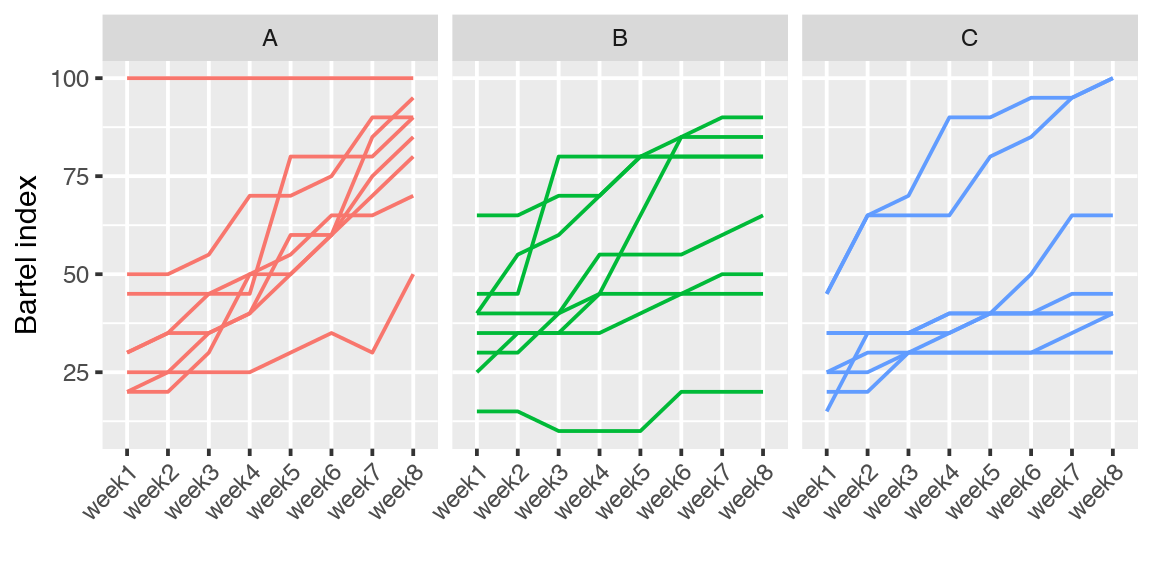
\includegraphics{hw_linear_reg_2_files/figure-latex/unnamed-chunk-10-1} \end{center}

\begin{Shaded}
\begin{Highlighting}[]
\NormalTok{polMD1 =}\StringTok{ }\KeywordTok{lm}\NormalTok{(}\DataTypeTok{data =}\NormalTok{ pollution, mort }\OperatorTok{~}\StringTok{ }\NormalTok{nox)}
\KeywordTok{plot}\NormalTok{(polMD1,}\DataTypeTok{which=}\DecValTok{1}\OperatorTok{:}\DecValTok{2}\NormalTok{)}
\end{Highlighting}
\end{Shaded}

\begin{center}\includegraphics{hw_linear_reg_2_files/figure-latex/unnamed-chunk-10-2} \end{center}

\begin{center}\includegraphics{hw_linear_reg_2_files/figure-latex/unnamed-chunk-10-3} \end{center}

\begin{Shaded}
\begin{Highlighting}[]
\KeywordTok{summary}\NormalTok{(polMD1)}
\end{Highlighting}
\end{Shaded}

\begin{verbatim}
## 
## Call:
## lm(formula = mort ~ nox, data = pollution)
## 
## Residuals:
##      Min       1Q   Median       3Q      Max 
## -148.654  -43.710    1.751   41.663  172.211 
## 
## Coefficients:
##             Estimate Std. Error t value Pr(>|t|)    
## (Intercept) 942.7115     9.0034 104.706   <2e-16 ***
## nox          -0.1039     0.1758  -0.591    0.557    
## ---
## Signif. codes:  0 '***' 0.001 '**' 0.01 '*' 0.05 '.' 0.1 ' ' 1
## 
## Residual standard error: 62.55 on 58 degrees of freedom
## Multiple R-squared:  0.005987,   Adjusted R-squared:  -0.01115 
## F-statistic: 0.3494 on 1 and 58 DF,  p-value: 0.5568
\end{verbatim}

Judging from the regression plot and the residual plot, the fit is
really bad.\newline

\begin{enumerate}
\def\labelenumi{\arabic{enumi}.}
\setcounter{enumi}{1}
\tightlist
\item
  Find an appropriate transformation that will result in data more
  appropriate for linear regression. Fit a regression to the transformed
  data and evaluate the new residual plot. \newline
\end{enumerate}

\begin{Shaded}
\begin{Highlighting}[]
\KeywordTok{ggplot}\NormalTok{(pollution)}\OperatorTok{+}\KeywordTok{aes}\NormalTok{(}\DataTypeTok{x =}\NormalTok{ nox)}\OperatorTok{+}\KeywordTok{geom_histogram}\NormalTok{(}\DataTypeTok{bins=}\DecValTok{30}\NormalTok{)}
\end{Highlighting}
\end{Shaded}

\begin{center}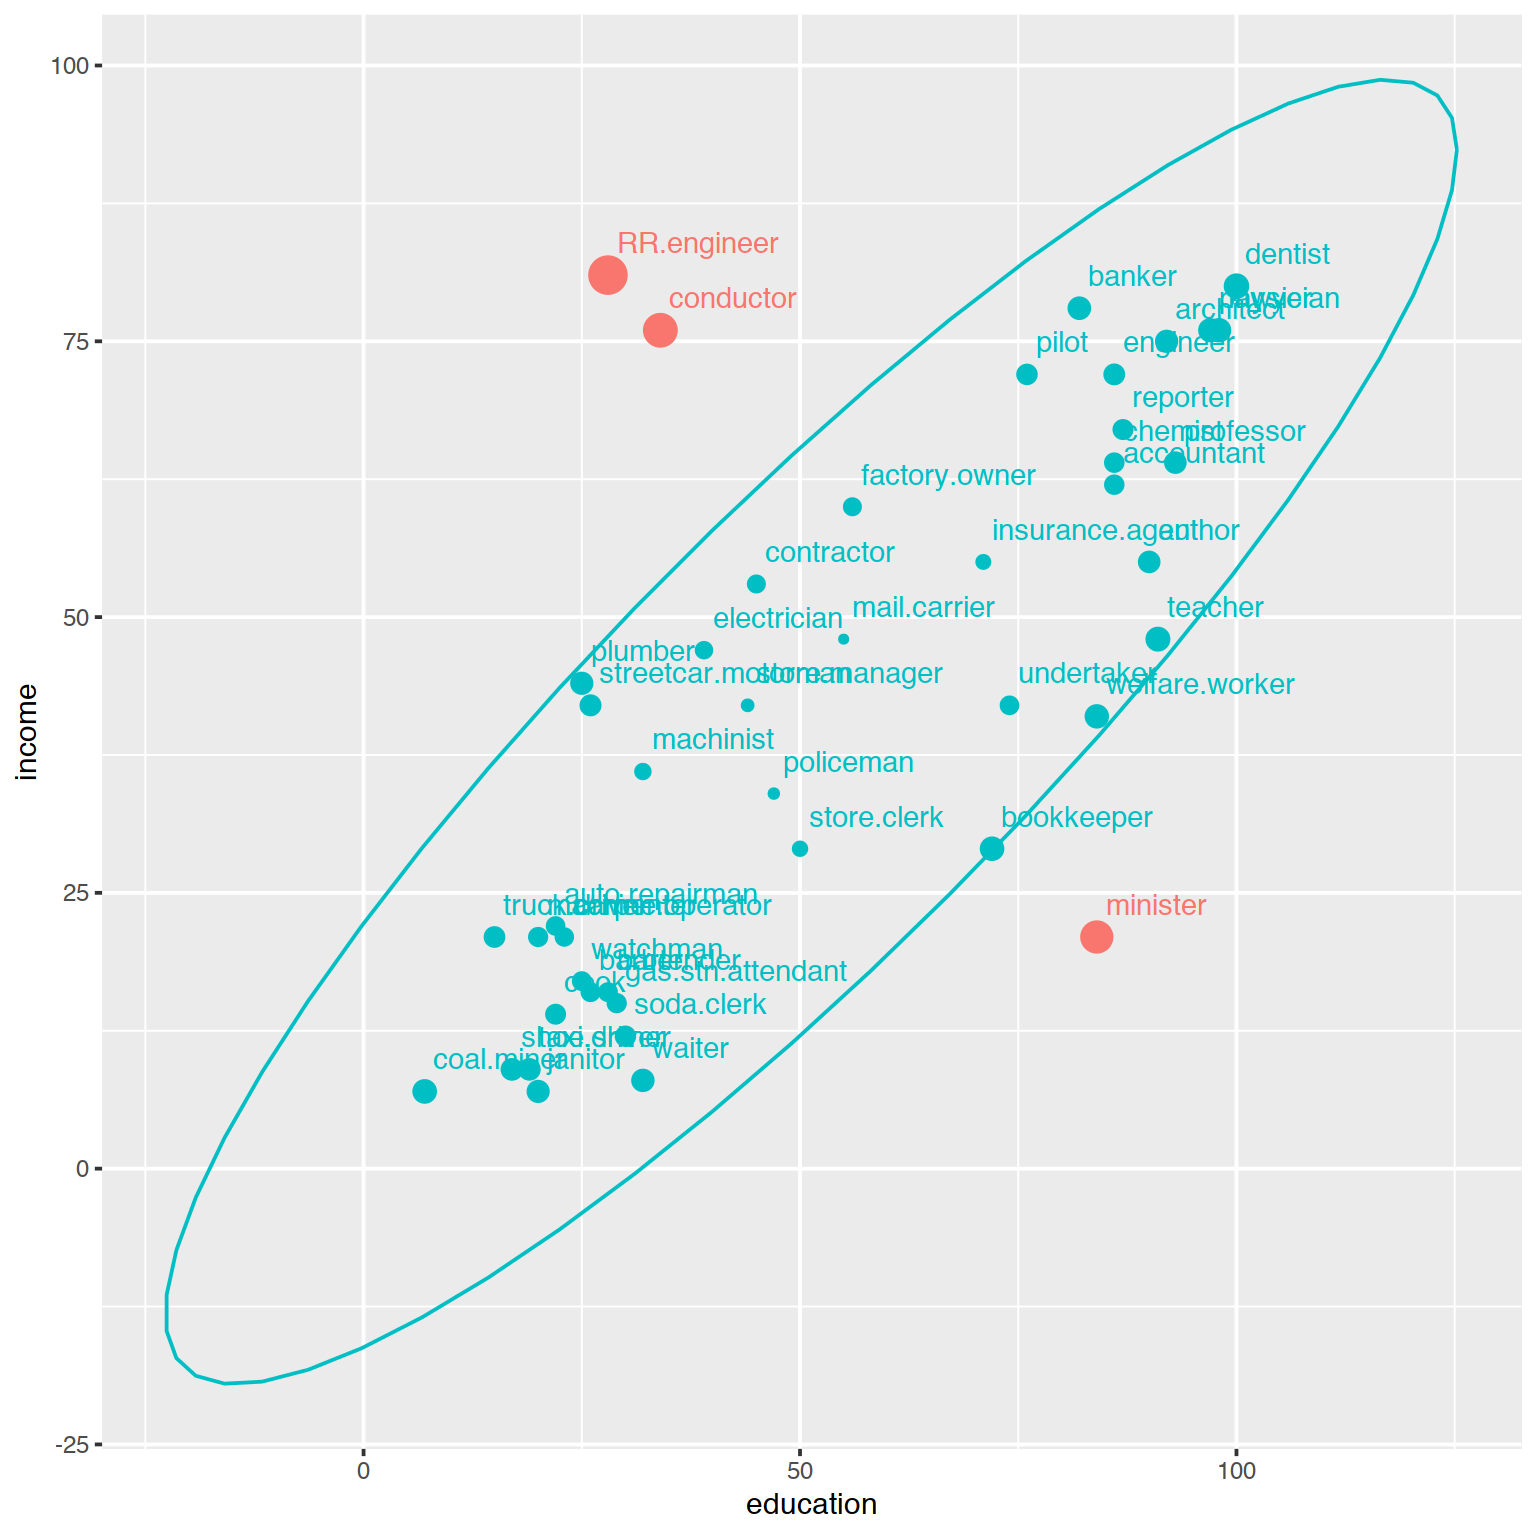
\includegraphics{hw_linear_reg_2_files/figure-latex/unnamed-chunk-11-1} \end{center}

\begin{Shaded}
\begin{Highlighting}[]
\KeywordTok{ggplot}\NormalTok{(pollution)}\OperatorTok{+}\KeywordTok{aes}\NormalTok{(}\DataTypeTok{x =} \KeywordTok{log}\NormalTok{(nox))}\OperatorTok{+}\KeywordTok{geom_histogram}\NormalTok{(}\DataTypeTok{bins=}\DecValTok{30}\NormalTok{)}
\end{Highlighting}
\end{Shaded}

\begin{center}\includegraphics{hw_linear_reg_2_files/figure-latex/unnamed-chunk-11-2} \end{center}

\begin{Shaded}
\begin{Highlighting}[]
\KeywordTok{ggplot}\NormalTok{(pollution)}\OperatorTok{+}\KeywordTok{aes}\NormalTok{(}\DataTypeTok{x =}\NormalTok{ mort)}\OperatorTok{+}\KeywordTok{geom_histogram}\NormalTok{(}\DataTypeTok{bins=}\DecValTok{30}\NormalTok{)}
\end{Highlighting}
\end{Shaded}

\begin{center}\includegraphics{hw_linear_reg_2_files/figure-latex/unnamed-chunk-11-3} \end{center}

\begin{Shaded}
\begin{Highlighting}[]
\KeywordTok{ggplot}\NormalTok{(pollution)}\OperatorTok{+}\KeywordTok{aes}\NormalTok{(}\DataTypeTok{x=}\KeywordTok{log}\NormalTok{(nox),}\DataTypeTok{y=}\NormalTok{mort)}\OperatorTok{+}\KeywordTok{geom_point}\NormalTok{()}\OperatorTok{+}\KeywordTok{geom_smooth}\NormalTok{(}\DataTypeTok{method=}\StringTok{'lm'}\NormalTok{,}\DataTypeTok{se=}\NormalTok{F)}
\end{Highlighting}
\end{Shaded}

\begin{center}\includegraphics{hw_linear_reg_2_files/figure-latex/unnamed-chunk-11-4} \end{center}

\begin{Shaded}
\begin{Highlighting}[]
\NormalTok{polMD2 =}\StringTok{ }\KeywordTok{lm}\NormalTok{(}\DataTypeTok{data =}\NormalTok{ pollution, mort }\OperatorTok{~}\StringTok{ }\KeywordTok{log}\NormalTok{(nox))}
\KeywordTok{plot}\NormalTok{(polMD2,}\DataTypeTok{which=}\DecValTok{1}\OperatorTok{:}\DecValTok{2}\NormalTok{)}
\end{Highlighting}
\end{Shaded}

\begin{center}\includegraphics{hw_linear_reg_2_files/figure-latex/unnamed-chunk-11-5} \end{center}

\begin{center}\includegraphics{hw_linear_reg_2_files/figure-latex/unnamed-chunk-11-6} \end{center}

\begin{Shaded}
\begin{Highlighting}[]
\KeywordTok{summary}\NormalTok{(polMD2)}
\end{Highlighting}
\end{Shaded}

\begin{verbatim}
## 
## Call:
## lm(formula = mort ~ log(nox), data = pollution)
## 
## Residuals:
##      Min       1Q   Median       3Q      Max 
## -167.140  -28.368    8.778   35.377  164.983 
## 
## Coefficients:
##             Estimate Std. Error t value Pr(>|t|)    
## (Intercept)  904.724     17.173  52.684   <2e-16 ***
## log(nox)      15.335      6.596   2.325   0.0236 *  
## ---
## Signif. codes:  0 '***' 0.001 '**' 0.01 '*' 0.05 '.' 0.1 ' ' 1
## 
## Residual standard error: 60.01 on 58 degrees of freedom
## Multiple R-squared:  0.08526,    Adjusted R-squared:  0.06949 
## F-statistic: 5.406 on 1 and 58 DF,  p-value: 0.02359
\end{verbatim}

The new model fits better to the dataset than the previous one. The
residual looks better, and the R-square had increased in a factor of
10.\newline

\begin{enumerate}
\def\labelenumi{\arabic{enumi}.}
\setcounter{enumi}{2}
\tightlist
\item
  Interpret the slope coefficient from the model you chose in 2.
\end{enumerate}

\begin{Shaded}
\begin{Highlighting}[]
\KeywordTok{summary}\NormalTok{(polMD2)}
\end{Highlighting}
\end{Shaded}

\begin{verbatim}
## 
## Call:
## lm(formula = mort ~ log(nox), data = pollution)
## 
## Residuals:
##      Min       1Q   Median       3Q      Max 
## -167.140  -28.368    8.778   35.377  164.983 
## 
## Coefficients:
##             Estimate Std. Error t value Pr(>|t|)    
## (Intercept)  904.724     17.173  52.684   <2e-16 ***
## log(nox)      15.335      6.596   2.325   0.0236 *  
## ---
## Signif. codes:  0 '***' 0.001 '**' 0.01 '*' 0.05 '.' 0.1 ' ' 1
## 
## Residual standard error: 60.01 on 58 degrees of freedom
## Multiple R-squared:  0.08526,    Adjusted R-squared:  0.06949 
## F-statistic: 5.406 on 1 and 58 DF,  p-value: 0.02359
\end{verbatim}

The intercept 904.724 is the mean mortality rate per 100,000 for nox
concentration of 1.\newline 4. Construct 99\% confidence interval for
slope coefficient from the model you chose in 2 and interpret them.

\begin{Shaded}
\begin{Highlighting}[]
\KeywordTok{kable}\NormalTok{(}\KeywordTok{t}\NormalTok{(}\KeywordTok{c}\NormalTok{(}\FloatTok{15.335}\DecValTok{-3}\OperatorTok{*}\FloatTok{6.596}\NormalTok{,}\FloatTok{15.335}\OperatorTok{+}\DecValTok{3}\OperatorTok{*}\FloatTok{6.596}\NormalTok{)),}\DataTypeTok{col.names =} \KeywordTok{c}\NormalTok{(}\StringTok{'99%CIlowerbound'}\NormalTok{,}\StringTok{'99%CIupperbound'}\NormalTok{),}\DataTypeTok{align =} \StringTok{'c'}\NormalTok{,}\DataTypeTok{format =} \StringTok{'html'}\NormalTok{)}
\end{Highlighting}
\end{Shaded}

99\%CIlowerbound

99\%CIupperbound

-4.453

35.123

if the same experiment can be done 100 times, one can expect 99 of the
times the true slope value lies within the rage of \(-4.453\) to
\(35.123\).\newline 5. Now fit a model predicting mortality rate using
levels of nitric oxides, sulfur dioxide, and hydrocarbons as inputs. Use
appropriate transformations when helpful. Plot the fitted regression
model and interpret the coefficients.

\begin{Shaded}
\begin{Highlighting}[]
\KeywordTok{ggplot}\NormalTok{(pollution)}\OperatorTok{+}\KeywordTok{aes}\NormalTok{(}\DataTypeTok{x =}\NormalTok{ so2)}\OperatorTok{+}\KeywordTok{geom_histogram}\NormalTok{(}\DataTypeTok{bins=}\DecValTok{30}\NormalTok{)}
\end{Highlighting}
\end{Shaded}

\begin{center}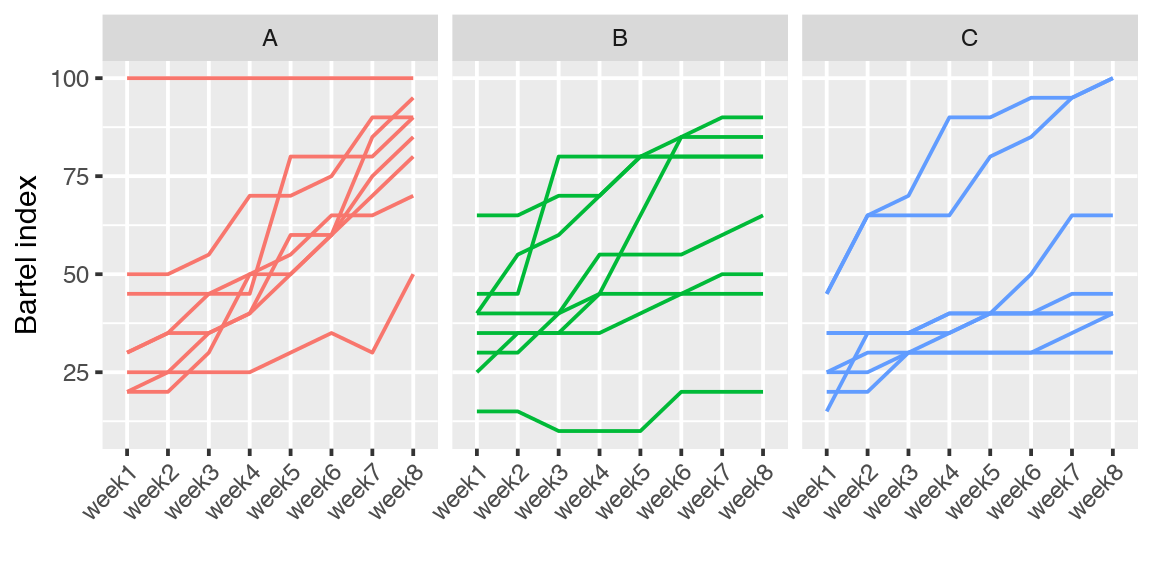
\includegraphics{hw_linear_reg_2_files/figure-latex/unnamed-chunk-14-1} \end{center}

\begin{Shaded}
\begin{Highlighting}[]
\KeywordTok{ggplot}\NormalTok{(pollution)}\OperatorTok{+}\KeywordTok{aes}\NormalTok{(}\DataTypeTok{x =}\NormalTok{ hc)}\OperatorTok{+}\KeywordTok{geom_histogram}\NormalTok{(}\DataTypeTok{bins=}\DecValTok{30}\NormalTok{)}
\end{Highlighting}
\end{Shaded}

\begin{center}\includegraphics{hw_linear_reg_2_files/figure-latex/unnamed-chunk-14-2} \end{center}

both \(SO^2\) and \(HC\) is heavily right skewed, so we can try log
transformation:

\begin{Shaded}
\begin{Highlighting}[]
\KeywordTok{ggplot}\NormalTok{(pollution)}\OperatorTok{+}\KeywordTok{aes}\NormalTok{(}\DataTypeTok{x =} \KeywordTok{log}\NormalTok{(so2))}\OperatorTok{+}\KeywordTok{geom_histogram}\NormalTok{(}\DataTypeTok{bins=}\DecValTok{30}\NormalTok{)}
\end{Highlighting}
\end{Shaded}

\begin{center}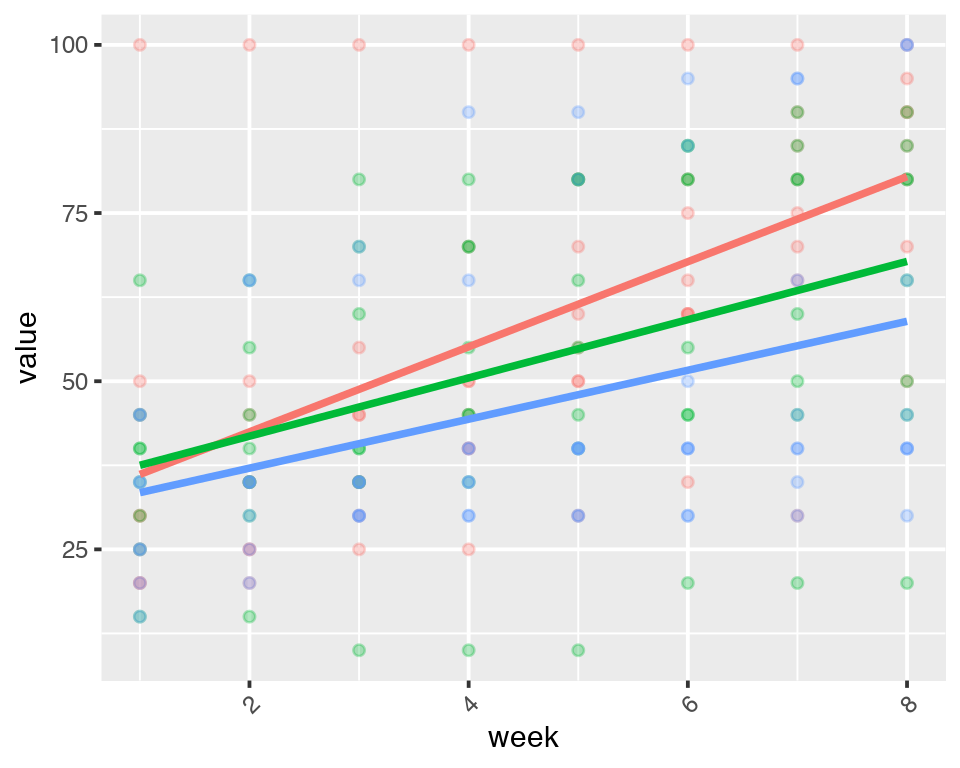
\includegraphics{hw_linear_reg_2_files/figure-latex/unnamed-chunk-15-1} \end{center}

\begin{Shaded}
\begin{Highlighting}[]
\KeywordTok{ggplot}\NormalTok{(pollution)}\OperatorTok{+}\KeywordTok{aes}\NormalTok{(}\DataTypeTok{x =} \KeywordTok{log}\NormalTok{(hc))}\OperatorTok{+}\KeywordTok{geom_histogram}\NormalTok{(}\DataTypeTok{bins=}\DecValTok{30}\NormalTok{)}
\end{Highlighting}
\end{Shaded}

\begin{center}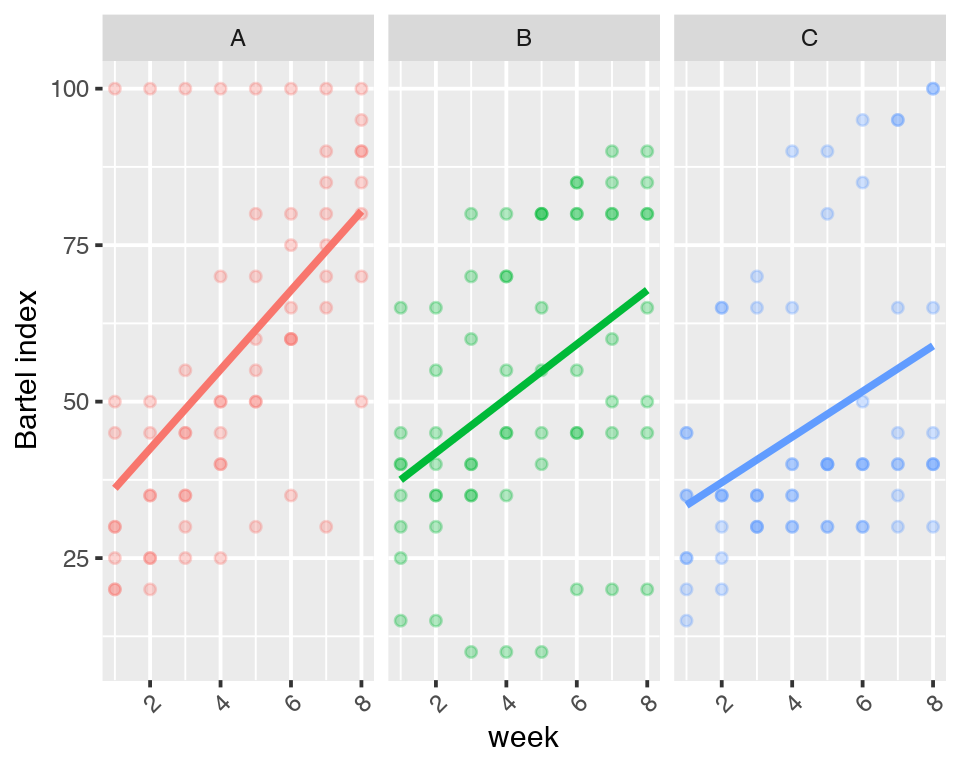
\includegraphics{hw_linear_reg_2_files/figure-latex/unnamed-chunk-15-2} \end{center}

log transformation looks fine, thus we can use this to perform our
prediction.

\begin{Shaded}
\begin{Highlighting}[]
\NormalTok{polMD3 =}\StringTok{ }\KeywordTok{lm}\NormalTok{(}\DataTypeTok{data =}\NormalTok{ pollution, mort }\OperatorTok{~}\StringTok{ }\KeywordTok{log}\NormalTok{(nox) }\OperatorTok{+}\StringTok{ }\KeywordTok{log}\NormalTok{(so2) }\OperatorTok{+}\StringTok{ }\KeywordTok{log}\NormalTok{(hc))}
\KeywordTok{summary}\NormalTok{(polMD3)}
\end{Highlighting}
\end{Shaded}

\begin{verbatim}
## 
## Call:
## lm(formula = mort ~ log(nox) + log(so2) + log(hc), data = pollution)
## 
## Residuals:
##     Min      1Q  Median      3Q     Max 
## -97.793 -34.728  -3.118  34.148 194.567 
## 
## Coefficients:
##             Estimate Std. Error t value Pr(>|t|)    
## (Intercept)  924.965     21.449  43.125  < 2e-16 ***
## log(nox)      58.336     21.751   2.682  0.00960 ** 
## log(so2)      11.762      7.165   1.642  0.10629    
## log(hc)      -57.300     19.419  -2.951  0.00462 ** 
## ---
## Signif. codes:  0 '***' 0.001 '**' 0.01 '*' 0.05 '.' 0.1 ' ' 1
## 
## Residual standard error: 54.36 on 56 degrees of freedom
## Multiple R-squared:  0.2752, Adjusted R-squared:  0.2363 
## F-statistic: 7.086 on 3 and 56 DF,  p-value: 0.0004044
\end{verbatim}

\begin{Shaded}
\begin{Highlighting}[]
\NormalTok{pollution1 =}\StringTok{ }\KeywordTok{mutate}\NormalTok{(pollution,}\DataTypeTok{predt =} \KeywordTok{predict}\NormalTok{(polMD3))}
\KeywordTok{ggplot}\NormalTok{(pollution1)}\OperatorTok{+}\KeywordTok{geom_point}\NormalTok{(}\DataTypeTok{mapping =} \KeywordTok{aes}\NormalTok{(}\DataTypeTok{x =} \KeywordTok{log}\NormalTok{(nox),}\DataTypeTok{y =}\NormalTok{ mort,}\DataTypeTok{color =} \StringTok{'Observed Mortality'}\NormalTok{))}\OperatorTok{+}\KeywordTok{geom_point}\NormalTok{(}\DataTypeTok{mapping =} \KeywordTok{aes}\NormalTok{(}\DataTypeTok{x =} \KeywordTok{log}\NormalTok{(nox),}\DataTypeTok{y =}\NormalTok{ predt,}\DataTypeTok{color=}\StringTok{'Predicted Value'}\NormalTok{))}
\end{Highlighting}
\end{Shaded}

\begin{center}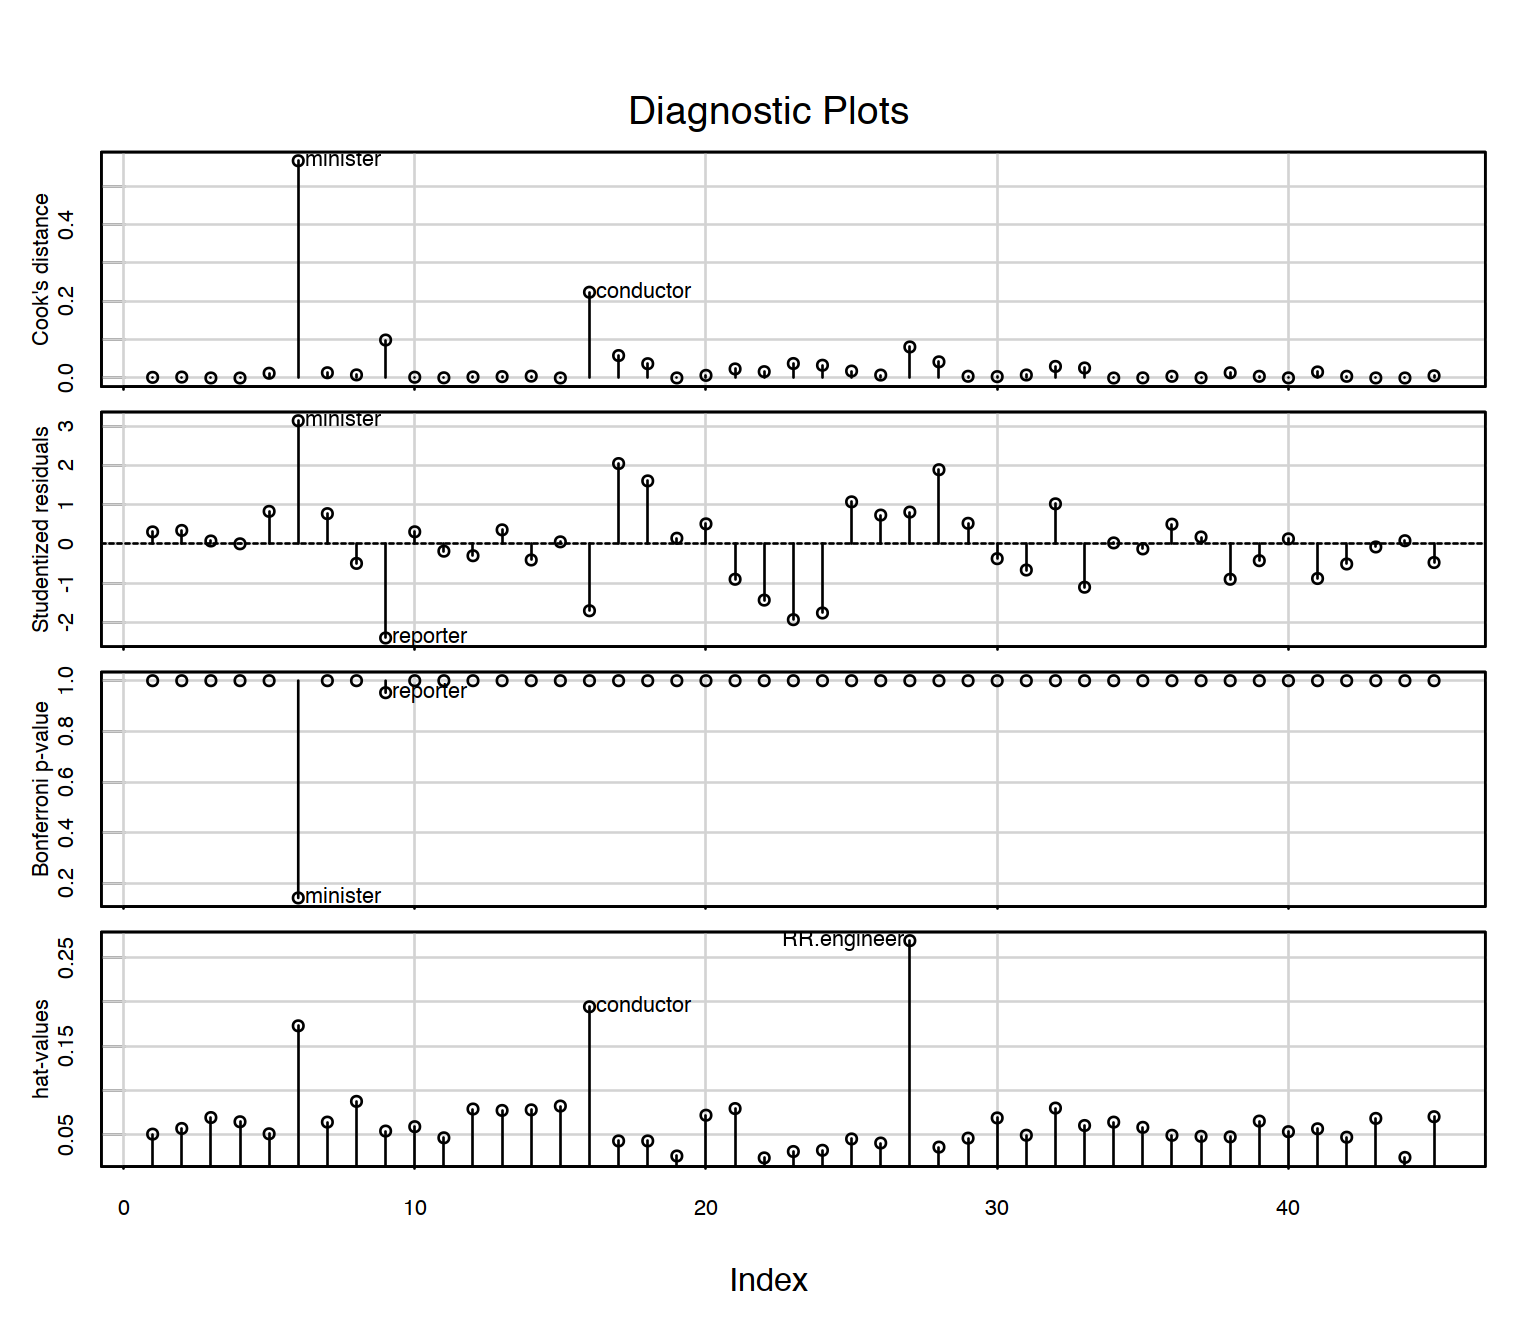
\includegraphics{hw_linear_reg_2_files/figure-latex/unnamed-chunk-16-1} \end{center}

Under this model, intercept means the average mortality rate is 924.965
per 100,000 people with nox, so2 and hc all equals to 1.\newline
coefficient for \(\ln nox\) means that for each 1 unit increase in
\(\ln nox\) one can averagly expect 58.336 increase in mortality rate
per 100,000 people\newline coefficient for \(\ln so_2\) means that for
each 1 unit increase in \(\ln so_2\) one can averagly expect 11.762
increase in mortality rate per 100,000 people\newline coefficient for
\(\ln hc\) means that for each 1 unit increase in \(\ln hc\) one can
averagly expect 57.300 decrese in mortality rate per 100,000
people\newline 6. Cross-validate: fit the model you chose above to the
first half of the data and then predict for the second half. (You used
all the data to construct the model in 4, so this is not really
cross-validation, but it gives a sense of how the steps of
cross-validation can be implemented.)

\begin{Shaded}
\begin{Highlighting}[]
\NormalTok{pol1 =}\StringTok{ }\KeywordTok{sample_frac}\NormalTok{(pollution,}\FloatTok{0.5}\NormalTok{,}\DataTypeTok{replace =}\NormalTok{ F)}
\NormalTok{pol2 =}\StringTok{ }\KeywordTok{setdiff}\NormalTok{(pollution,pol1)}\OperatorTok\KeywordTok{select}\NormalTok{(nox,so2,hc,mort)}

\NormalTok{polMD4 =}\StringTok{ }\KeywordTok{lm}\NormalTok{(}\DataTypeTok{data =}\NormalTok{ pol1, mort }\OperatorTok{~}\StringTok{ }\KeywordTok{log}\NormalTok{(nox) }\OperatorTok{+}\StringTok{ }\KeywordTok{log}\NormalTok{(so2) }\OperatorTok{+}\StringTok{ }\KeywordTok{log}\NormalTok{(hc))}
\KeywordTok{summary}\NormalTok{(polMD4)}\OperatorTok{$}\NormalTok{r.squared}
\end{Highlighting}
\end{Shaded}

\begin{verbatim}
## [1] 0.5661568
\end{verbatim}

\begin{Shaded}
\begin{Highlighting}[]
\NormalTok{pol2 =}\StringTok{ }\KeywordTok{mutate}\NormalTok{(pol2, }\DataTypeTok{predt =} \KeywordTok{predict}\NormalTok{(}\DataTypeTok{object =}\NormalTok{ polMD4,}\DataTypeTok{newdata =}\NormalTok{ pol2))}\OperatorTok\KeywordTok{mutate}\NormalTok{(}\DataTypeTok{y =}\NormalTok{ mort }\OperatorTok{-}\StringTok{ }\KeywordTok{mean}\NormalTok{(mort))}\OperatorTok\KeywordTok{mutate}\NormalTok{(}\DataTypeTok{err =}\NormalTok{ mort }\OperatorTok{-}\StringTok{ }\NormalTok{predt)}

\CommentTok{##R-squared on test set}
\NormalTok{(}\DecValTok{1}\OperatorTok{-}\NormalTok{((pol2}\OperatorTok{$}\NormalTok{err}\OperatorTok\NormalTok{pol2}\OperatorTok{$}\NormalTok{err)}\OperatorTok{/}\NormalTok{(pol2}\OperatorTok{$}\NormalTok{y}\OperatorTok\NormalTok{pol2}\OperatorTok{$}\NormalTok{y)))[}\DecValTok{1}\NormalTok{]}
\end{Highlighting}
\end{Shaded}

\begin{verbatim}
## [1] -0.171854
\end{verbatim}

\hypertarget{study-of-teenage-gambling-in-britain}{%
\subsubsection{Study of teenage gambling in
Britain}\label{study-of-teenage-gambling-in-britain}}

\begin{enumerate}
\def\labelenumi{\arabic{enumi}.}
\tightlist
\item
  Fit a linear regression model with gamble as the response and the
  other variables as predictors and interpret the coefficients. Make
  sure you rename and transform the variables to improve the
  interpretability of your regression model.
\end{enumerate}

\begin{Shaded}
\begin{Highlighting}[]
\CommentTok{## construct log income and log gambling}
\NormalTok{teengamb1 =}\StringTok{ }\KeywordTok{mutate}\NormalTok{(teengamb1,}\DataTypeTok{log.in =} \KeywordTok{log}\NormalTok{(income))}\OperatorTok\KeywordTok{mutate}\NormalTok{(}\DataTypeTok{log.gamb =} \KeywordTok{log}\NormalTok{(gamble))}
\CommentTok{## choosing log.income and sex to build model}
\NormalTok{teenMD =}\StringTok{ }\KeywordTok{lm}\NormalTok{(}\DataTypeTok{data =}\NormalTok{ teengamb1,log.gamb }\OperatorTok{~}\StringTok{ }\NormalTok{sex }\OperatorTok{+}\StringTok{ }\NormalTok{log.in }\OperatorTok{+}\StringTok{ }\NormalTok{sex }\OperatorTok{*}\StringTok{ }\NormalTok{log.in)}
\NormalTok{teenMDcoef =}\StringTok{ }\KeywordTok{exp}\NormalTok{(}\KeywordTok{as.tibble}\NormalTok{(}\KeywordTok{summary}\NormalTok{(teenMD)}\OperatorTok{$}\NormalTok{coef)[,}\DecValTok{1}\NormalTok{])}
\KeywordTok{kable}\NormalTok{(}\KeywordTok{t}\NormalTok{(teenMDcoef),}\DataTypeTok{format =} \StringTok{'html'}\NormalTok{,}\DataTypeTok{digits =} \DecValTok{3}\NormalTok{, }\DataTypeTok{align =} \StringTok{'c'}\NormalTok{,}\DataTypeTok{col.names =} \KeywordTok{c}\NormalTok{(}\StringTok{'Intercept'}\NormalTok{,}\StringTok{'Gender'}\NormalTok{,}\StringTok{'Log.in'}\NormalTok{,}\StringTok{'Gen : Log.in'}\NormalTok{))}
\end{Highlighting}
\end{Shaded}

Intercept

Gender

Log.in

Gen : Log.in

Estimate

2.091

1.373

3.545

0.19

\begin{Shaded}
\begin{Highlighting}[]
\KeywordTok{kable}\NormalTok{(}\KeywordTok{summary}\NormalTok{(teenMD)}\OperatorTok{$}\NormalTok{coef,}\DataTypeTok{format =} \StringTok{'html'}\NormalTok{, }\DataTypeTok{digits =} \DecValTok{3}\NormalTok{, }\DataTypeTok{align =} \StringTok{'c'}\NormalTok{)}
\end{Highlighting}
\end{Shaded}

Estimate

Std. Error

t value

Pr(\textgreater{}\textbar{}t\textbar{})

(Intercept)

0.738

0.600

1.229

0.226

sex

0.317

1.224

0.259

0.797

log.in

1.265

0.392

3.232

0.003

sex:log.in

-1.659

0.828

-2.005

0.052

\begin{Shaded}
\begin{Highlighting}[]
\KeywordTok{ggplot}\NormalTok{(teengamb1)}\OperatorTok{+}\KeywordTok{aes}\NormalTok{(}\DataTypeTok{x =}\NormalTok{ log.in, }\DataTypeTok{y=}\NormalTok{log.gamb,}\DataTypeTok{color =} \KeywordTok{as.factor}\NormalTok{(sex))}\OperatorTok{+}\KeywordTok{geom_point}\NormalTok{()}\OperatorTok{+}\KeywordTok{geom_smooth}\NormalTok{(}\DataTypeTok{method =} \StringTok{'lm'}\NormalTok{,}\DataTypeTok{se=}\NormalTok{F)}
\end{Highlighting}
\end{Shaded}

\begin{center}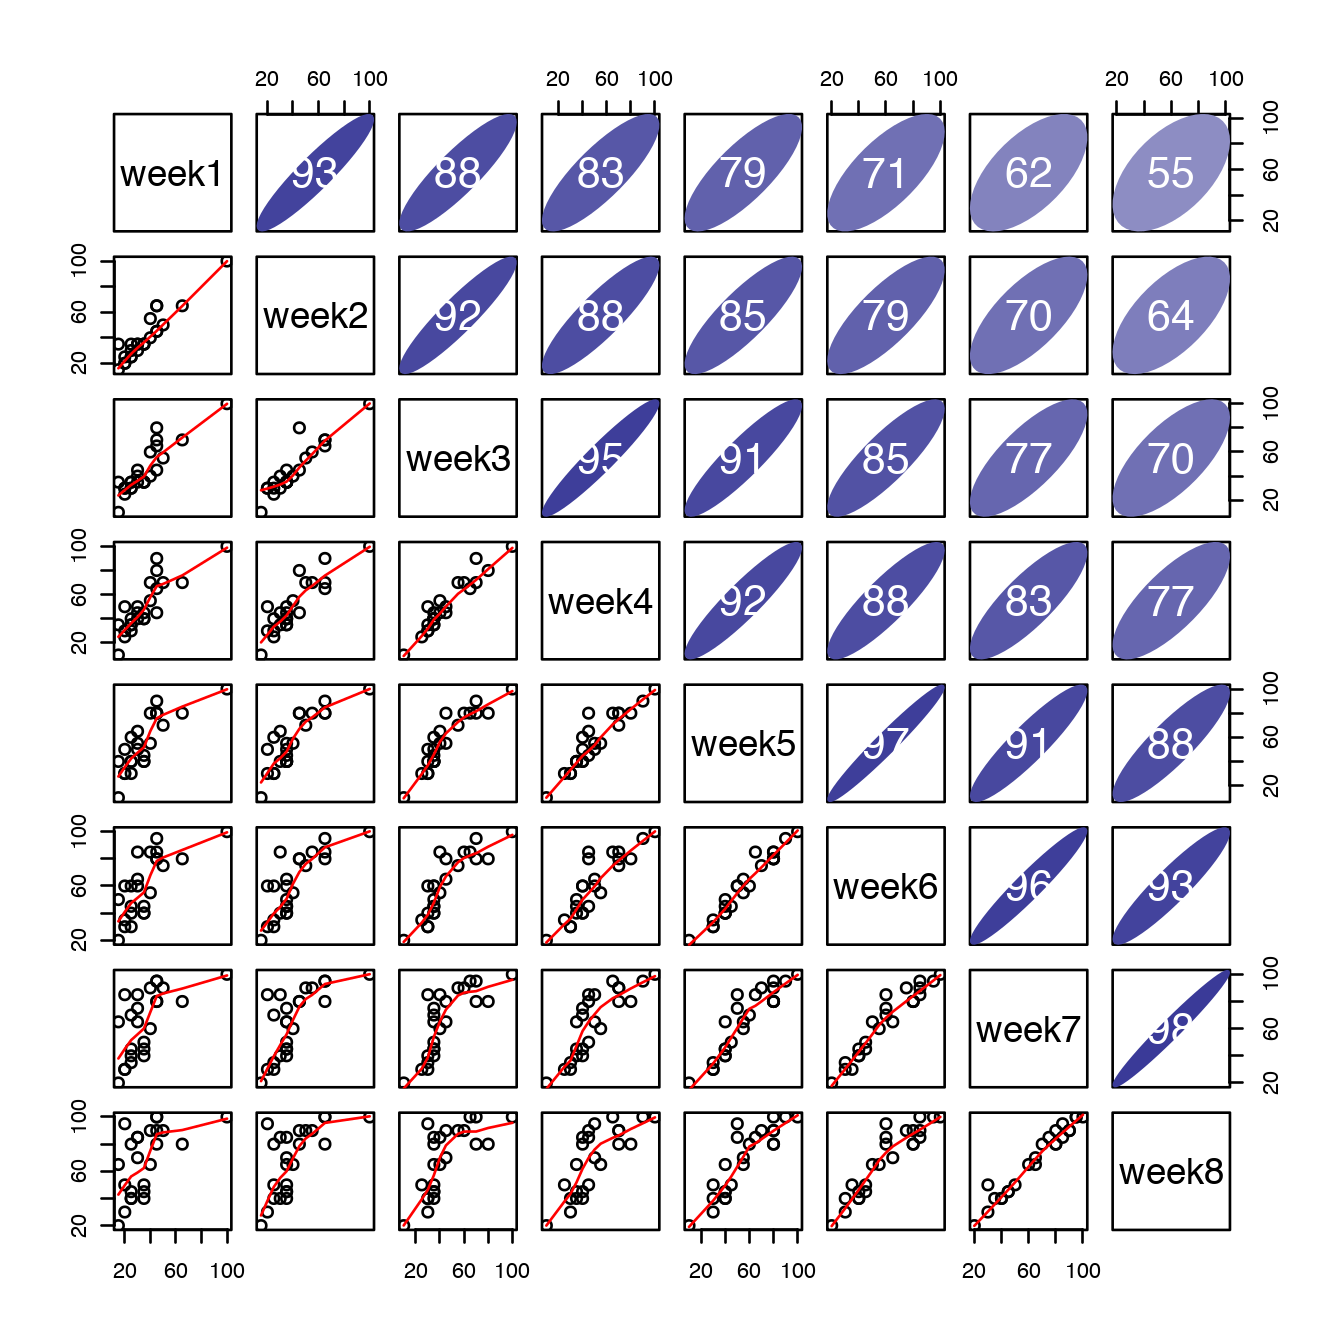
\includegraphics{hw_linear_reg_2_files/figure-latex/unnamed-chunk-19-1} \end{center}

The intercept means the mean for male with 1 income per week, will
gamble 2.091 per year in pounds\newline The coefficient for gender means
the for female with 1 income per week is predicted to put 37.3\% more on
gambling per year\newline The coefficient for log.income means that for
male, unit increase in log income per week will increase gambing per
year by 254.5\%\newline The coefficient for Gen:log.in means that for
female, the increase in gambling per year will decrease by 81\% compare
to male\newline 2. Create a 95\% confidence interval for each of the
estimated coefficients and discuss how you would interpret this
uncertainty.

\begin{Shaded}
\begin{Highlighting}[]
\NormalTok{gambsum =}\StringTok{ }\KeywordTok{as_tibble}\NormalTok{(}\KeywordTok{summary}\NormalTok{(teenMD)}\OperatorTok{$}\NormalTok{coef)}\OperatorTok\KeywordTok{select}\NormalTok{(}\DecValTok{1}\OperatorTok{:}\DecValTok{2}\NormalTok{)}\OperatorTok\StringTok{`}\DataTypeTok{colnames<-}\StringTok{`}\NormalTok{(}\KeywordTok{c}\NormalTok{(}\StringTok{'Est'}\NormalTok{,}\StringTok{'StandardError'}\NormalTok{))}\OperatorTok\KeywordTok{mutate}\NormalTok{(}\DataTypeTok{lower95CI =}\NormalTok{ Est}\DecValTok{-2}\OperatorTok{*}\NormalTok{StandardError)}\OperatorTok\KeywordTok{mutate}\NormalTok{(}\DataTypeTok{upper95CI =}\NormalTok{ Est}\OperatorTok{+}\DecValTok{2}\OperatorTok{*}\NormalTok{StandardError)}\OperatorTok\StringTok{`}\DataTypeTok{rownames<-}\StringTok{`}\NormalTok{(}\KeywordTok{rownames}\NormalTok{(}\KeywordTok{summary}\NormalTok{(teenMD)}\OperatorTok{$}\NormalTok{coef))}
\end{Highlighting}
\end{Shaded}

\begin{verbatim}
## Warning: Setting row names on a tibble is deprecated.
\end{verbatim}

\begin{Shaded}
\begin{Highlighting}[]
\KeywordTok{kable}\NormalTok{(gambsum,}\DataTypeTok{format =} \StringTok{'html'}\NormalTok{,}\DataTypeTok{digits =} \DecValTok{2}\NormalTok{,}\DataTypeTok{align =} \StringTok{'c'}\NormalTok{)}
\end{Highlighting}
\end{Shaded}

Est

StandardError

lower95CI

upper95CI

(Intercept)

0.74

0.60

-0.46

1.94

sex

0.32

1.22

-2.13

2.77

log.in

1.27

0.39

0.48

2.05

sex:log.in

-1.66

0.83

-3.31

0.00

\begin{enumerate}
\def\labelenumi{\arabic{enumi}.}
\setcounter{enumi}{2}
\tightlist
\item
  Predict the amount that a male with average status, income and verbal
  score would gamble along with an appropriate 95\% CI. Repeat the
  prediction for a male with maximal values of status, income and verbal
  score. Which CI is wider and why is this result expected?
\end{enumerate}

\begin{Shaded}
\begin{Highlighting}[]
\NormalTok{teengamb1 =}\StringTok{ }\KeywordTok{mutate}\NormalTok{(teengamb1,}\DataTypeTok{mean.status =}\NormalTok{ status}\OperatorTok{-}\KeywordTok{mean}\NormalTok{(status))}\OperatorTok\KeywordTok{mutate}\NormalTok{(}\DataTypeTok{mean.logincome =}\NormalTok{ log.in }\OperatorTok{-}\StringTok{ }\KeywordTok{mean}\NormalTok{(log.in))}\OperatorTok\KeywordTok{mutate}\NormalTok{(}\DataTypeTok{mean.verbal =}\NormalTok{ verbal }\OperatorTok{-}\StringTok{ }\KeywordTok{mean}\NormalTok{(verbal))}\OperatorTok\KeywordTok{mutate}\NormalTok{(}\DataTypeTok{max.status =}\NormalTok{ status }\OperatorTok{-}\StringTok{ }\KeywordTok{max}\NormalTok{(status))}\OperatorTok\KeywordTok{mutate}\NormalTok{(}\DataTypeTok{max.logincome =}\NormalTok{ log.in }\OperatorTok{-}\StringTok{ }\KeywordTok{max}\NormalTok{(log.in))}\OperatorTok\KeywordTok{mutate}\NormalTok{(}\DataTypeTok{max.verbal =}\NormalTok{ verbal }\OperatorTok{-}\StringTok{ }\KeywordTok{max}\NormalTok{(verbal))}
\NormalTok{teenMD2 =}\StringTok{ }\KeywordTok{lm}\NormalTok{(}\DataTypeTok{data =}\NormalTok{ teengamb1,log.gamb }\OperatorTok{~}\StringTok{ }\NormalTok{mean.status }\OperatorTok{+}\StringTok{ }\NormalTok{mean.logincome }\OperatorTok{+}\StringTok{ }\NormalTok{mean.verbal)}
\NormalTok{teenMD3 =}\StringTok{ }\KeywordTok{lm}\NormalTok{(}\DataTypeTok{data =}\NormalTok{ teengamb1,log.gamb }\OperatorTok{~}\StringTok{ }\NormalTok{max.status }\OperatorTok{+}\StringTok{ }\NormalTok{max.logincome }\OperatorTok{+}\StringTok{ }\NormalTok{max.verbal)}
\NormalTok{sum1 =}\StringTok{ }\KeywordTok{t}\NormalTok{(}\KeywordTok{as_tibble}\NormalTok{(}\KeywordTok{summary}\NormalTok{(teenMD2)}\OperatorTok{$}\NormalTok{coef[}\DecValTok{1}\NormalTok{,}\DecValTok{1}\OperatorTok{:}\DecValTok{2}\NormalTok{]))}
\CommentTok{##lower95CI for mean}
\NormalTok{sum1[}\DecValTok{1}\NormalTok{]}\OperatorTok{-}\DecValTok{2}\OperatorTok{*}\NormalTok{sum1[}\DecValTok{2}\NormalTok{]}
\end{Highlighting}
\end{Shaded}

\begin{verbatim}
## [1] 1.129144
\end{verbatim}

\begin{Shaded}
\begin{Highlighting}[]
\CommentTok{##upper95CI for mean}
\NormalTok{sum1[}\DecValTok{1}\NormalTok{]}\OperatorTok{+}\DecValTok{2}\OperatorTok{*}\NormalTok{sum1[}\DecValTok{2}\NormalTok{]}
\end{Highlighting}
\end{Shaded}

\begin{verbatim}
## [1] 2.238994
\end{verbatim}

\begin{Shaded}
\begin{Highlighting}[]
\NormalTok{sum2 =}\StringTok{ }\KeywordTok{t}\NormalTok{(}\KeywordTok{as_tibble}\NormalTok{(}\KeywordTok{summary}\NormalTok{(teenMD3)}\OperatorTok{$}\NormalTok{coef[}\DecValTok{1}\NormalTok{,}\DecValTok{1}\OperatorTok{:}\DecValTok{2}\NormalTok{]))}
\CommentTok{##lower95CI for mean}
\NormalTok{sum2[}\DecValTok{1}\NormalTok{]}\OperatorTok{-}\DecValTok{2}\OperatorTok{*}\NormalTok{sum2[}\DecValTok{2}\NormalTok{]}
\end{Highlighting}
\end{Shaded}

\begin{verbatim}
## [1] 1.822091
\end{verbatim}

\begin{Shaded}
\begin{Highlighting}[]
\CommentTok{##upper95CI for mean}
\NormalTok{sum2[}\DecValTok{1}\NormalTok{]}\OperatorTok{+}\DecValTok{2}\OperatorTok{*}\NormalTok{sum2[}\DecValTok{2}\NormalTok{]}
\end{Highlighting}
\end{Shaded}

\begin{verbatim}
## [1] 5.49428
\end{verbatim}

The maximal CI is wider, because locally there is fewer points than the
mean ones, which results in bigger variance. \#\#\# School expenditure
and test scores from USA in 1994-95

\begin{Shaded}
\begin{Highlighting}[]
\NormalTok{sat =}\StringTok{ }\NormalTok{sat}
\end{Highlighting}
\end{Shaded}

\begin{enumerate}
\def\labelenumi{\arabic{enumi}.}
\tightlist
\item
  Fit a model with total sat score as the outcome and expend, ratio and
  salary as predictors. Make necessary transformation in order to
  improve the interpretability of the model. Interpret each of the
  coefficient.
\end{enumerate}

\begin{Shaded}
\begin{Highlighting}[]
\KeywordTok{hist}\NormalTok{(sat}\OperatorTok{$}\NormalTok{total)}
\end{Highlighting}
\end{Shaded}

\begin{center}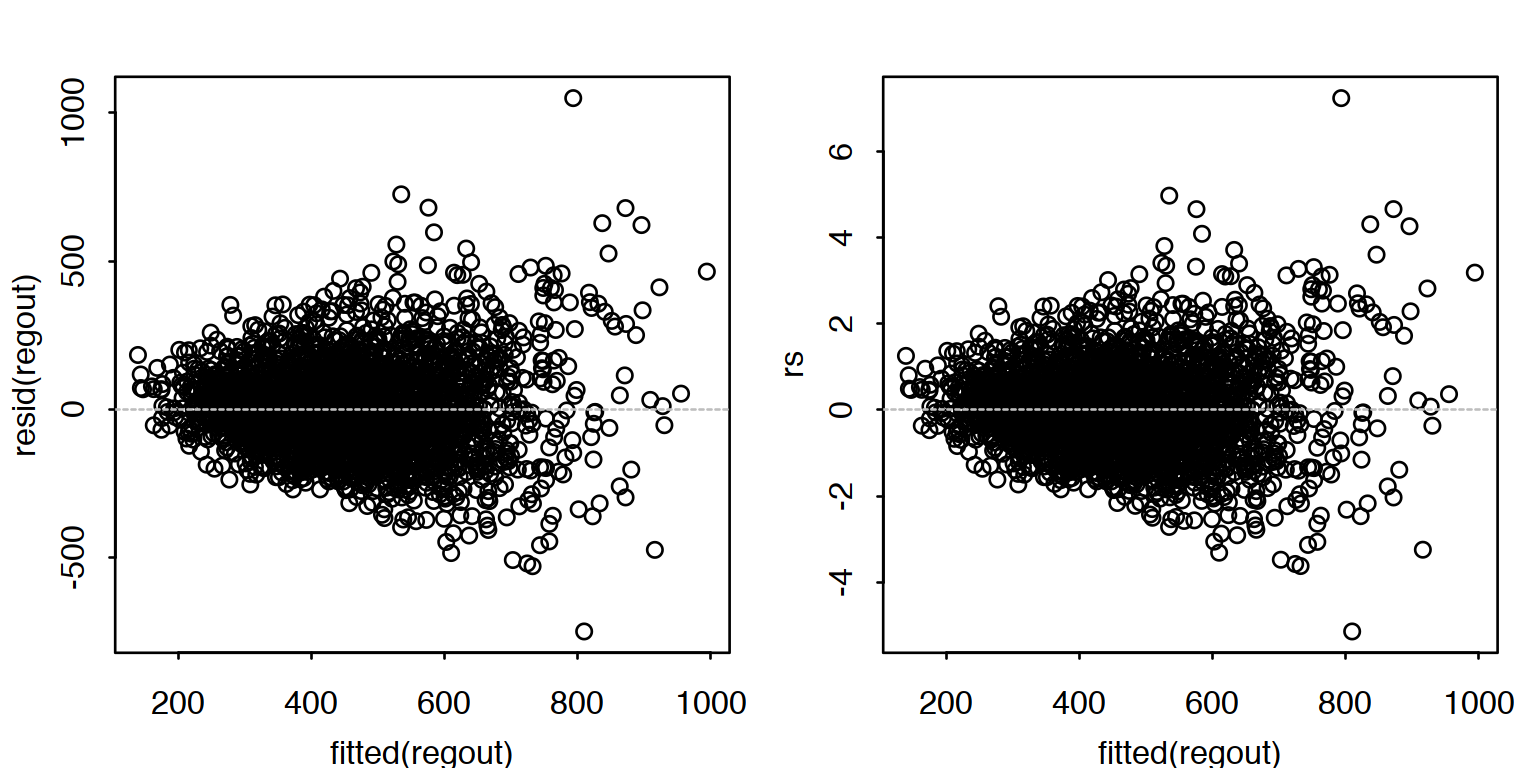
\includegraphics{hw_linear_reg_2_files/figure-latex/unnamed-chunk-23-1} \end{center}

\begin{Shaded}
\begin{Highlighting}[]
\KeywordTok{hist}\NormalTok{(}\KeywordTok{log}\NormalTok{(sat}\OperatorTok{$}\NormalTok{expend))}
\end{Highlighting}
\end{Shaded}

\begin{center}\includegraphics{hw_linear_reg_2_files/figure-latex/unnamed-chunk-23-2} \end{center}

\begin{Shaded}
\begin{Highlighting}[]
\KeywordTok{hist}\NormalTok{(}\KeywordTok{log}\NormalTok{(sat}\OperatorTok{$}\NormalTok{ratio))}
\end{Highlighting}
\end{Shaded}

\begin{center}\includegraphics{hw_linear_reg_2_files/figure-latex/unnamed-chunk-23-3} \end{center}

\begin{Shaded}
\begin{Highlighting}[]
\KeywordTok{hist}\NormalTok{(}\KeywordTok{log}\NormalTok{(sat}\OperatorTok{$}\NormalTok{salary))}
\end{Highlighting}
\end{Shaded}

\begin{center}\includegraphics{hw_linear_reg_2_files/figure-latex/unnamed-chunk-23-4} \end{center}

\begin{Shaded}
\begin{Highlighting}[]
\NormalTok{sat1 =}\StringTok{ }\KeywordTok{mutate}\NormalTok{(sat,}\DataTypeTok{log.expend =} \KeywordTok{log}\NormalTok{(expend))}\OperatorTok\KeywordTok{mutate}\NormalTok{(}\DataTypeTok{log.ratio =} \KeywordTok{log}\NormalTok{(ratio))}\OperatorTok\KeywordTok{mutate}\NormalTok{(}\DataTypeTok{log.salary =} \KeywordTok{log}\NormalTok{(salary))}\OperatorTok\KeywordTok{mutate}\NormalTok{(}\DataTypeTok{meanlog.expend =}\NormalTok{ log.expend}\OperatorTok{-}\KeywordTok{mean}\NormalTok{(log.expend))}\OperatorTok\KeywordTok{mutate}\NormalTok{(}\DataTypeTok{meanlog.ratio =}\NormalTok{ log.ratio}\OperatorTok{-}\KeywordTok{mean}\NormalTok{(log.ratio))}\OperatorTok\KeywordTok{mutate}\NormalTok{(}\DataTypeTok{meanlog.salary =}\NormalTok{ log.salary}\OperatorTok{-}\KeywordTok{mean}\NormalTok{(log.salary))}\OperatorTok\KeywordTok{mutate}\NormalTok{(}\DataTypeTok{meantakers =}\NormalTok{ takers}\OperatorTok{-}\KeywordTok{mean}\NormalTok{(takers))}
\NormalTok{satMD1 =}\StringTok{ }\KeywordTok{lm}\NormalTok{(}\DataTypeTok{data =}\NormalTok{ sat1, total }\OperatorTok{~}\StringTok{ }\NormalTok{meanlog.expend }\OperatorTok{+}\StringTok{ }\NormalTok{meanlog.ratio }\OperatorTok{+}\StringTok{ }\NormalTok{meanlog.salary)}
\KeywordTok{summary}\NormalTok{(satMD1)}
\end{Highlighting}
\end{Shaded}

\begin{verbatim}
## 
## Call:
## lm(formula = total ~ meanlog.expend + meanlog.ratio + meanlog.salary, 
##     data = sat1)
## 
## Residuals:
##      Min       1Q   Median       3Q      Max 
## -141.883  -45.280   -8.312   47.040  125.150 
## 
## Coefficients:
##                Estimate Std. Error t value Pr(>|t|)    
## (Intercept)     965.920      9.627 100.332   <2e-16 ***
## meanlog.expend   92.895    133.651   0.695   0.4905    
## meanlog.ratio   117.352    121.224   0.968   0.3381    
## meanlog.salary -311.093    161.183  -1.930   0.0598 .  
## ---
## Signif. codes:  0 '***' 0.001 '**' 0.01 '*' 0.05 '.' 0.1 ' ' 1
## 
## Residual standard error: 68.08 on 46 degrees of freedom
## Multiple R-squared:  0.2229, Adjusted R-squared:  0.1722 
## F-statistic: 4.397 on 3 and 46 DF,  p-value: 0.008403
\end{verbatim}

\begin{Shaded}
\begin{Highlighting}[]
\KeywordTok{plot}\NormalTok{(satMD1,}\DataTypeTok{which =} \DecValTok{1}\OperatorTok{:}\DecValTok{2}\NormalTok{)}
\end{Highlighting}
\end{Shaded}

\begin{center}\includegraphics{hw_linear_reg_2_files/figure-latex/unnamed-chunk-23-5} \end{center}

\begin{center}\includegraphics{hw_linear_reg_2_files/figure-latex/unnamed-chunk-23-6} \end{center}

intercept means average SAT score for average log.expend, average
log.ratio and average log.salary\newline The coef of meanlog.expend for
every unit increase in log expend, SAT scores would expect to increase
92.895.\newline The coef of meanlog.ratio means for every unit increase
in log ratio, SAT scores would expect to increase 117.352\newline the
coef of meanlog.salary means for every unit increse in log salary, SAT
scores would expect to decrese 311.093\newline

\begin{enumerate}
\def\labelenumi{\arabic{enumi}.}
\setcounter{enumi}{1}
\tightlist
\item
  Construct 99\% CI for each coefficient and discuss what you see.
\end{enumerate}

\begin{Shaded}
\begin{Highlighting}[]
\NormalTok{satsum =}\StringTok{ }\KeywordTok{as_tibble}\NormalTok{(}\KeywordTok{summary}\NormalTok{(satMD1)}\OperatorTok{$}\NormalTok{coef)}\OperatorTok\KeywordTok{select}\NormalTok{(}\DecValTok{1}\OperatorTok{:}\DecValTok{2}\NormalTok{)}\OperatorTok\StringTok{`}\DataTypeTok{colnames<-}\StringTok{`}\NormalTok{(}\KeywordTok{c}\NormalTok{(}\StringTok{'Est'}\NormalTok{,}\StringTok{'StandardError'}\NormalTok{))}\OperatorTok\KeywordTok{mutate}\NormalTok{(}\DataTypeTok{lower95CI =}\NormalTok{ Est}\DecValTok{-2}\OperatorTok{*}\NormalTok{StandardError)}\OperatorTok\KeywordTok{mutate}\NormalTok{(}\DataTypeTok{upper95CI =}\NormalTok{ Est}\OperatorTok{+}\DecValTok{2}\OperatorTok{*}\NormalTok{StandardError)}\OperatorTok\StringTok{`}\DataTypeTok{rownames<-}\StringTok{`}\NormalTok{(}\KeywordTok{rownames}\NormalTok{(}\KeywordTok{summary}\NormalTok{(satMD1)}\OperatorTok{$}\NormalTok{coef))}
\end{Highlighting}
\end{Shaded}

\begin{verbatim}
## Warning: Setting row names on a tibble is deprecated.
\end{verbatim}

\begin{Shaded}
\begin{Highlighting}[]
\KeywordTok{kable}\NormalTok{(satsum,}\DataTypeTok{format =} \StringTok{'html'}\NormalTok{,}\DataTypeTok{digits =} \DecValTok{2}\NormalTok{,}\DataTypeTok{align =} \StringTok{'c'}\NormalTok{)}
\end{Highlighting}
\end{Shaded}

Est

StandardError

lower95CI

upper95CI

(Intercept)

965.92

9.63

946.67

985.17

meanlog.expend

92.90

133.65

-174.41

360.20

meanlog.ratio

117.35

121.22

-125.10

359.80

meanlog.salary

-311.09

161.18

-633.46

11.27

the takeaway is that, there might not be an actual correlation between
SAT scores and the predictors\newline 3. Now add takers to the model.
Compare the fitted model to the previous model and discuss which of the
model seem to explain the outcome better?

\begin{Shaded}
\begin{Highlighting}[]
\NormalTok{satMD2 =}\StringTok{ }\KeywordTok{lm}\NormalTok{(}\DataTypeTok{data =}\NormalTok{ sat1, total }\OperatorTok{~}\StringTok{ }\NormalTok{meanlog.expend }\OperatorTok{+}\StringTok{ }\NormalTok{meanlog.ratio }\OperatorTok{+}\StringTok{ }\NormalTok{meanlog.salary }\OperatorTok{+}\StringTok{ }\NormalTok{meantakers)}
\KeywordTok{anova}\NormalTok{(satMD1,satMD2)}
\end{Highlighting}
\end{Shaded}

\begin{verbatim}
## Analysis of Variance Table
## 
## Model 1: total ~ meanlog.expend + meanlog.ratio + meanlog.salary
## Model 2: total ~ meanlog.expend + meanlog.ratio + meanlog.salary + meantakers
##   Res.Df    RSS Df Sum of Sq      F    Pr(>F)    
## 1     46 213174                                  
## 2     45  48030  1    165144 154.73 3.657e-16 ***
## ---
## Signif. codes:  0 '***' 0.001 '**' 0.01 '*' 0.05 '.' 0.1 ' ' 1
\end{verbatim}

\begin{Shaded}
\begin{Highlighting}[]
\KeywordTok{summary}\NormalTok{(satMD1)}
\end{Highlighting}
\end{Shaded}

\begin{verbatim}
## 
## Call:
## lm(formula = total ~ meanlog.expend + meanlog.ratio + meanlog.salary, 
##     data = sat1)
## 
## Residuals:
##      Min       1Q   Median       3Q      Max 
## -141.883  -45.280   -8.312   47.040  125.150 
## 
## Coefficients:
##                Estimate Std. Error t value Pr(>|t|)    
## (Intercept)     965.920      9.627 100.332   <2e-16 ***
## meanlog.expend   92.895    133.651   0.695   0.4905    
## meanlog.ratio   117.352    121.224   0.968   0.3381    
## meanlog.salary -311.093    161.183  -1.930   0.0598 .  
## ---
## Signif. codes:  0 '***' 0.001 '**' 0.01 '*' 0.05 '.' 0.1 ' ' 1
## 
## Residual standard error: 68.08 on 46 degrees of freedom
## Multiple R-squared:  0.2229, Adjusted R-squared:  0.1722 
## F-statistic: 4.397 on 3 and 46 DF,  p-value: 0.008403
\end{verbatim}

\begin{Shaded}
\begin{Highlighting}[]
\KeywordTok{summary}\NormalTok{(satMD2)}
\end{Highlighting}
\end{Shaded}

\begin{verbatim}
## 
## Call:
## lm(formula = total ~ meanlog.expend + meanlog.ratio + meanlog.salary + 
##     meantakers, data = sat1)
## 
## Residuals:
##     Min      1Q  Median      3Q     Max 
## -92.613 -20.727   0.343  13.809  67.984 
## 
## Coefficients:
##                Estimate Std. Error t value Pr(>|t|)    
## (Intercept)    965.9200     4.6202 209.063  < 2e-16 ***
## meanlog.expend  15.9424    64.4382   0.247    0.806    
## meanlog.ratio  -79.9294    60.2999  -1.326    0.192    
## meanlog.salary  71.8433    83.2543   0.863    0.393    
## meantakers      -2.9199     0.2347 -12.439 3.66e-16 ***
## ---
## Signif. codes:  0 '***' 0.001 '**' 0.01 '*' 0.05 '.' 0.1 ' ' 1
## 
## Residual standard error: 32.67 on 45 degrees of freedom
## Multiple R-squared:  0.8249, Adjusted R-squared:  0.8093 
## F-statistic:    53 on 4 and 45 DF,  p-value: < 2.2e-16
\end{verbatim}

clearly from the anova test, adding takers significantly improve the fit
\# Conceptual exercises.

\hypertarget{special-purpose-transformations}{%
\subsubsection{Special-purpose
transformations:}\label{special-purpose-transformations}}

For a study of congressional elections, you would like a measure of the
relative amount of money raised by each of the two major-party
candidates in each district. Suppose that you know the amount of money
raised by each candidate; label these dollar values \(D_i\) and \(R_i\).
You would like to combine these into a single variable that can be
included as an input variable into a model predicting vote share for the
Democrats.

Discuss the advantages and disadvantages of the following measures:

\begin{itemize}
\tightlist
\item
  The simple difference, \(D_i-R_i\)

  \begin{itemize}
  \tightlist
  \item
    advantages includes

    \begin{itemize}
    \tightlist
    \item
      substraction provides quick classification from plus and minus
      sign.
    \item
      know the exact difference
    \end{itemize}
  \item
    disadvantages includes

    \begin{itemize}
    \tightlist
    \item
      zero and negative value can be a problem for future
      transformation.
    \item
      lose the knowledge of how close or how different the two party
      is(eg: 5500\$ difference with each raised over 1mil vs.~500\$
      difference with each raised 5000ish)
    \end{itemize}
  \end{itemize}
\item
  The ratio, \(D_i/R_i\)

  \begin{itemize}
  \tightlist
  \item
    advantages includes

    \begin{itemize}
    \tightlist
    \item
      quick classification comparing to `1'
    \item
      always greater than zero, easy to transform
    \end{itemize}
  \item
    disadvantages includes

    \begin{itemize}
    \tightlist
    \item
      lose the exact amount of difference in raised money
    \item
      when \(R_i\) isa small, increases rapidly, not evenly distributed.
    \end{itemize}
  \end{itemize}
\item
  The difference on the logarithmic scale, \(log D_i-log R_i\)

  \begin{itemize}
  \tightlist
  \item
    is esentailly taking log on \(D_i/R_i\)
  \item
    resolve some distribution issue, but still lose the exact amount
    difference info.
  \end{itemize}
\item
  The relative proportion, \(D_i/(D_i+R_i)\).

  \begin{itemize}
  \tightlist
  \item
    well organized, scale from 0 to 1.
  \item
    but lose info on actual amount
  \end{itemize}
\end{itemize}

\hypertarget{transformation}{%
\subsubsection{Transformation}\label{transformation}}

For observed pair of \(\mathrm{x}\) and \(\mathrm{y}\), we fit a simple
regression model
\[\mathrm{y}=\alpha + \beta \mathrm{x} + \mathrm{\epsilon}\] which
results in estimates \(\hat{\alpha}=1\), \(\hat{\beta}=0.9\),
\(SE(\hat{\beta})=0.03\), \(\hat{\sigma}=2\) and \(r=0.3\).

\begin{enumerate}
\def\labelenumi{\arabic{enumi}.}
\item
  Suppose that the explanatory variable values in a regression are
  transformed according to the \(\mathrm{x}^{\star}=\mathrm{x}-10\) and
  that \(\mathrm{y}\) is regressed on \(\mathrm{x}^{\star}\). Without
  redoing the regression calculation in detail, find
  \(\hat{\alpha}^{\star}\), \(\hat{\beta}^{\star}\),
  \(\hat{\sigma}^{\star}\), and \(r^{\star}\). What happens to these
  quantities when \(\mathrm{x}^{\star}=10\mathrm{x}\) ? When
  \(\mathrm{x}^{\star}=10(\mathrm{x}-1)\)?\newline When
  \(\mathrm{x}^{\star}=\mathrm{x}-10\)
  \[\alpha^{\star} = \alpha - 10 \cdot \beta\] \[\beta^{\star} = \beta\]
  \[\sigma^{\star} = \sigma\] When \(\mathrm{x}^{\star}=10\mathrm{x}\)
  \[\alpha^{\star} = \alpha\] \[\beta^{\star} = \beta/10\]
  \[\sigma^{\star} = \sigma\] When
  \(\mathrm{x}^{\star}=10(\mathrm{x}-1)\)
  \[\alpha^{\star} = \alpha-\beta\] \[\beta^{\star} = \beta/10\]
  \[\sigma^{\star} = \sigma\]
\item
  Now suppose that the response variable scores are transformed
  according to the formula \(\mathrm{y}^{\star\star}= \mathrm{y}+10\)
  and that \(\mathrm{y}^{\star\star}\) is regressed on \(\mathrm{x}\).
  Without redoing the regression calculation in detail, find
  \(\hat{\alpha}^{\star\star}\), \(\hat{\beta}^{\star\star}\),
  \(\hat{\sigma}^{\star\star}\), and \(r^{\star\star}\). What happens to
  these quantities when \(\mathrm{y}^{\star\star}=5\mathrm{y}\) ? When
  \(\mathrm{y}^{\star\star}=5(\mathrm{y}+2)\)?\newline When
  \(\mathrm{y}^{\star\star}=a(\mathrm{y}+b) , a\neq0\)
  \[\alpha^{\star\star} = a(\alpha+b)\]
  \[\beta^{\star\star} = a\cdot\beta\]
  \[\sigma^{\star\star} = \sqrt{a}\cdot\sigma\]
\item
  In general, how are the results of a simple regression analysis
  affected by linear transformations of \(\mathrm{y}\) and
  \(\mathrm{x}\)? rules:\newline multiplication on \(x\) equals to
  divide the \(\beta\) term, substraction of \(x\) equals to add
  substraction \(\times \beta\) to the intercept\newline multiplication
  on \(y\) equals to multiplication on all coeficients, substraction on
  \(y\) equals to substract on intercept
\item
  Suppose that the explanatory variable values in a regression are
  transformed according to the \(\mathrm{x}^{\star}=10(\mathrm{x}-1)\)
  and that \(\mathrm{y}\) is regressed on \(\mathrm{x}^{\star}\).
  Without redoing the regression calculation in detail, find
  \(SE(\hat{\beta}^{\star})\) and
  \(t^{\star}_0= \hat{\beta}^{\star}/SE(\hat{\beta}^{\star})\).
\item
  Now suppose that the response variable scores are transformed
  according to the formula \(\mathrm{y}^{\star\star}=5(\mathrm{y}+2)\)
  and that \(\mathrm{y}^{\star\star}\) is regressed on \(\mathrm{x}\).
  Without redoing the regression calculation in detail, find
  \(SE(\hat{\beta}^{\star\star})\) and
  \(t^{\star\star}_0= \hat{\beta}^{\star\star}/SE(\hat{\beta}^{\star\star})\).
\item
  In general, how are the hypothesis tests and confidence intervals for
  \(\beta\) affected by linear transformations of \(\mathrm{y}\) and
  \(\mathrm{x}\)?
\end{enumerate}

\hypertarget{feedback-comments-etc.}{%
\section{Feedback comments etc.}\label{feedback-comments-etc.}}

If you have any comments about the homework, or the class, please write
your feedback here. We love to hear your opinions.

modeling took too much time to finish, and they are not really different
from one another, conceptual questions are much more fun


\end{document}
